% Report for group 15
% Eugenio Piccini
% Francesco Davide Bossio
% Mirko Legnini
%
\documentclass[a4paper,11pt,oneside]{report}
\usepackage[latin1]{inputenc}
\usepackage[english]{babel}
\usepackage{amsfonts}
\usepackage{amsmath}
\usepackage{amssymb,amsmath,color}
\usepackage{cite}
\usepackage{graphicx}
\usepackage{float}
\usepackage{titlesec}
\usepackage{placeins}
\usepackage{animate}

\titleformat{\chapter}[display]   
{\normalfont\huge\bfseries}{\chaptertitlename\ \thechapter}{20pt}{\Huge}   
\titlespacing*{\chapter}{0pt}{-40pt}{40pt}

% this alters "before" spacing (the second length argument) to 0
\titlespacing*{\chapter}{0pt}{0pt}{40pt}

\begin{document}
\pagestyle{myheadings}

%%%%%%%%%%% Cover %%%%%%%%%%%
\thispagestyle{empty}                                                 
\begin{center}                                                            
    \vspace{5mm}
    {\LARGE UNIVERSIT\`A DI BOLOGNA} \\                       
      \vspace{5mm}
\end{center}
\begin{center}
  
\includegraphics[scale=.27]{figs/logo_unibo.png}
\end{center}
\begin{center}
      \vspace{5mm}
      {\LARGE School of Engineering} \\
        \vspace{3mm}
      {\Large Master Degree in Automation Engineering} \\
      \vspace{20mm}
      {\LARGE Optimal Control} \\
      \vspace{5mm}{\Large\textbf{Course Project \#1 $-$ Group 15 \\ Optimal Control of a Vehicle}}                  
      \vspace{15mm}
\end{center}
\begin{flushleft}                                                                              
     {\large Professor: \textbf{\@ Giuseppe Notarstefano}} \\        
      \vspace{13mm}
\end{flushleft}
\begin{flushright}
      {\large Students:\\} Eugenio Piccini \\
       Francesco Davide Bossio \\
       Mirko Legnini\\
\end{flushright}        
\begin{center}
\vfill
      {\large Academic year \@2023/2024} \\
\end{center}



\newpage
\thispagestyle{empty}

%%%%%%%%%%% Abstract %%%%%%%%%%%%
\begin{center}
\chapter*{}
\thispagestyle{empty}
{\Huge \textbf{Abstract}}\\
This project deals with the design and implementation of an 
optimal control law for a simple bicycle model with static load transfer.\\
Tasks involve dynamics discretization, trajectory generation 
both with step and smooth change between two equilibria,
trajectory tracking via LQR and MPC algorithms and at last an animation of the vehicle
following the trajectory generated with the LQR algorithm.
\vspace{15mm}
\end{center}

\tableofcontents \thispagestyle{empty}
% \listoffigures\thispagestyle{empty}

%%%%%%%%%% Introduction %%%%%%%%%%
\chapter*{Introduction}
\addcontentsline{toc}{chapter}{Introduction}
In this project, we are required to design an optimal trajectory, so a sequence of state-input pairs (\textbf{x},\textbf{u})
that satisfies the system dynamics and minimize a designed cost function, for a vehicle modeled by a bicycle model.\\
In order to achieve this goal we will work on four different tasks:
\begin{itemize}
	\item Task 0 - Problem setup:
Discretize and find the expression for the gradients of the system dynamics and code them. 

    \item Task 1 - Step trajectory generation:
Compute two equilibria of the system and define a reference (step) curve between the two.
Compute the optimal transition between the two exploiting the Newton's-like algorithm for optimal control. 

      \item Task 2 - Smooth trajectory generation:
Use the same algorithm as above to track a smooth reference curve.

    \item Task 3 - Trajectory tracking via LQR:
Linearize the model around the optimal trajectory obtained before and define the optimal feedback controller
to perform trajectory tracking via LQR algorithm.

    \item Task 4 - Trajectory tracking via MPC:
Perform trajectory tracking now using the MPC algorithm.

    \item Task 5 - Animation:
Produce a simple animation of the vehicle executing Task 3.
\end{itemize}

\section*{Contributions}



%%%%%%%%%% Chapter Title %%%%%%%%%   

\chapter{Task 0 - Problem setup}

The aim of this task is to discretize the system dynamics, compute the gradients of the functions and code them.

\section{State space and control inputs}
The system can be modeled as a simple bicycle model,
as shown in Figure \ref{fig:Bicycle}.

\begin{figure}[htp]
\centering
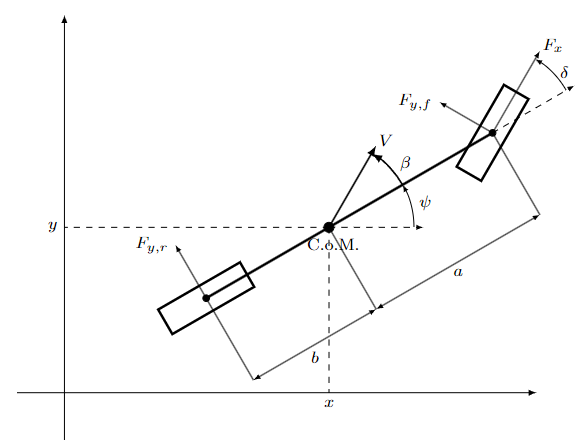
\includegraphics[width=0.5\textwidth]{figs/Bycicle.png}
\caption{Bicycle model}
\label{fig:Bicycle}
\end{figure}

The state space variables are \[ x = [x, y, \psi, V, \beta, \dot{\psi}]^T\] where: $x$ and $y$ represent the position of the center of mass [CoM],
$\psi$ the angle between the horizontal and the chassis, $V$ the velocity of the CoM with respect to the inertial frame, $\beta$ the angle between the chassis and the velocity vector, 
$\dot{\psi}$ the angular rate of changes associated to $\psi$.
The input is \[u = [\delta, F_x]^T\] where $\delta$ is the steering angle and $F_x$ is the force applied by the wheels.

\bigskip
The dynamic model is described by:
\[
\begin{cases}
    \dot{x} &= V\cos\beta\cos\psi - V\sin\beta\sin\psi \\
    \dot{y} &= V\cos\beta\sin\psi + V\sin\beta\cos\psi \\
    m\dot{V} &= F_{y,r} \sin\beta + F_x \cos(\beta - \delta) + F_{y,f}\sin(\beta - \delta) \\
    \dot{\beta} &= \frac{1}{mV}(F_{y,r}\cos\beta + F_{y,f}\cos(\beta - \delta) - F_x\sin(\beta - \delta)) - \dot{\psi} \\
    I_z\ddot{\psi} &= (F_x\sin\delta + F_{y,f}\cos\delta)a - F_{y,r}b\\
\end{cases}
\]

The lateral forces \( F_{y,f} \) and \( F_{y,r} \) can be found as:

\[
\begin{aligned}
    F_{y,f} &= \mu F_{z,f} \beta_f \\
    F_{y,r} &= \mu F_{z,r} \beta_r
\end{aligned}
\]

where \( \beta_f \) and \( \beta_r \) are the front and rear sideslip angles:

\[
\begin{aligned}
    \beta_f = \delta - \frac{V\sin\beta + a\dot{\psi}}{V\cos\beta} \\
    \beta_r = -\frac{V\sin\beta - b\dot{\psi}}{V\cos\beta}
\end{aligned}
\]

The vertical forces on the front and rear wheel can be found as:

\[
\begin{aligned}
    F_{z,f} &= \frac{mgb}{a + b} \\
    F_{z,r} &= \frac{mga}{a + b}
\end{aligned}
\]

The mechanical parameters of the car are: 

\begin{center}
\begin{tabular}{ |c|c|c| } 
 \hline
 m: mass of the car & 1480 & [Kg] \\ 
 $I_z$: inertia of the car & 1950 & $[kg m^2]$ \\ 
 a: distance between rear wheel and CoM & 1.421 & [m]\\ 
 b: distance between front wheel and CoM & 1.029 & [m]\\ 
 $\mu$: friction coefficient & 1 & [nodim]\\ 
 g: acceleration due to gravity & 9.81 & $[m/s^2]$\\ 
 \hline
\end{tabular}
\end{center}


\section{Forward Euler discretization}
In order to write the discrete-time state-space equations, we consider the discrete time version of the bicycle model dynamics, discretized via forward Euler: 
\[
x_{t+1}  = x_t + \delta f_{CT} (x_t, u_t, t)\\
\]

where $\delta > 0$ is a sufficiently small discretization step and $f_{CT} (\cdot,\cdot,\cdot)$ is the continuous-time dynamics. In particular, we choose $\delta = 10^{-2}$. 


We obtain the following discrete-time state-space equations: 
\[
\begin{cases}
    x_{t+1} &= x_t + \delta(V\cos\beta\cos\psi - V\sin\beta\sin\psi) \\
    y_{t+1} &= y_t + \delta(V\cos\beta\sin\psi + V\sin\beta\cos\psi) \\
    \psi_{t+1} &= \psi_t + \delta(\dot{\psi}) \\
    V_{t+1} &= v_t + \delta\left(\frac{1}{m}\left(F_{y,r}\sin\beta + F_x\cos(\beta - \delta) + F_{y,f}\sin(\beta - \delta)\right)\right) \\
    \beta_{t+1} &= \beta_t + \delta\left(\frac{1}{mV}\left(F_{y,r}\cos\beta + F_{y,f}\cos(\beta - \delta) - F_x\sin(\beta - \delta)\right) - (\dot{\psi})\right) \\
    \dot{\psi}_{t+1} &= \dot{\psi}_t + \delta\left(\frac{1}{I_z}\left((F_x\sin\delta + F_{y,f}\cos\delta)a - F_{y,r}b\right)\right)
\end{cases} 
\]

Next, since we are dealing with a non-linear system that is time-invariant, it is necessary to linearize the model by taking its gradient with respect to the state, which is defined as the transpose of the Jacobian Matrix:
\[
    \nabla_1 f(x,u) = \left[\nabla_1 f_1(x,u), \nabla_1 f_2(x,u), \nabla_1 f_3(x,u), \nabla_1 f_4(x,u), \nabla_1 f_5(x,u), \nabla_1 f_6(x,u)\right]
\]

After that, we compute the gradient of our dynamics with respect to our input:
\[
    \nabla_2 f(x,u) = [\nabla_2 f_1(x,u), \nabla_2 f_2(x,u), \nabla_2 f_3(x,u), \nabla_2 f_4(x,u), \nabla_2 f_5(x,u), \nabla_2 f_6(x,u)]
\]

In principle, in order to implement a precise Newton's method, we would also need to compute the Hessian of the dynamics. However, since we used the regularized Newton's method, we don't need these computation as only the hessians of the costs will be needed. We will discuss other implications for this choice in the next chapter. 
\chapter{Task 1 - Newton's method on step trajectory}
The aim of this task is to compute a desired input state curve and create an optimal trajectory that minimizes the cost with respect to this desired curve. 

\section{Equilibrium computation}
The desired curve is required to start and end in equilibrium points for the system. We don't consider the trivial equilibrium for a set position, namely 
\begin{align*}
 f_1(x_t,u_t)=0 \\
 f_2(x_t,u_t)=0 \\
 f_3(x_t,u_t)=0 \\
\end{align*}
Which implies $x_4=x_5=x_6=0$, as they wouldn't give us an insightful understanding of the system behavior.
We instead considered the so called cornering equilibria of the system, for which the following holds:
\begin{align*}
 f_1(x_t,u_t) \neq 0 \\
 f_2(x_t,u_t) \neq 0 \\
 f_3(x_t,u_t) \neq 0 \\
 f_4(x_t,u_t)=0 \\
 f_5(x_t,u_t)=0 \\
 f_6(x_t,u_t)=0 
\end{align*}
This trajectories can be characterized as either a uniform linear or a uniform circular movement. 
Since the states $x_1, x_2, x_3$ do not have a role in the dynamics for the last three states, as they are just integrated from the latter, we can find these cornering equilibria by studying the reduced system

\begin{align*}
	m \dot{x_4} = F_{y,r} \sin x_5 + u_2 \cos (x_5 - u_1) + F_{y,f} \sin (x_5 - u_1) \\
    \dot{x_5} = \frac{1} {m x_4} (F_{y,r} \cos x_5 + F_{y,f} \cos(x_5 - u_1) - u_2 \sin (x_5 - u_1))-x_6
    \\
    I_z \dot{x_6} = (u_1 \sin u_1 + F_{y,f}\cos u_1 )a - F_{y,r} b   
\end{align*}
 
Which is a three equation system in five variables. This means we have two degrees of freedom in choosing the desired equilibrium variables, and find the others by solving the system. 
We decided to set the velocity module $x_4$ and the velocity angle $x_5$. We've found the other equilibrium values for the system with a zero finding method, using \texttt{sp.fsolve} from the scipy toolbox. \\
By imposing $(x_4^1, x_5^1)=(8, 0)$ and $(x_4^1, x_5^1)=(12, \frac{\pi}{6})$ we have found the cornering equilibrium pairs for the system dynamics.
\\ We proceeded by integrating the dynamics, which is useful both to check the values and to create the desired curve. The complete desired curve is computed by concatenating the two subtrajectories. 
\begin{figure}[!h]
	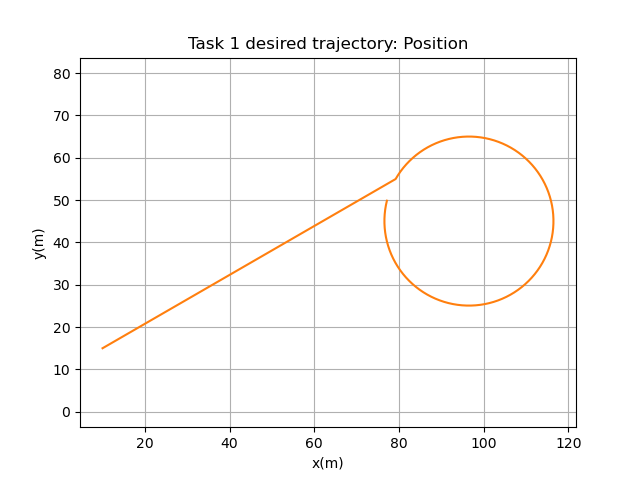
\includegraphics[width=\linewidth]{figs/destraj.png}
	\caption{Desired step position trajectory}
\end{figure} 

\begin{figure}[!h]
	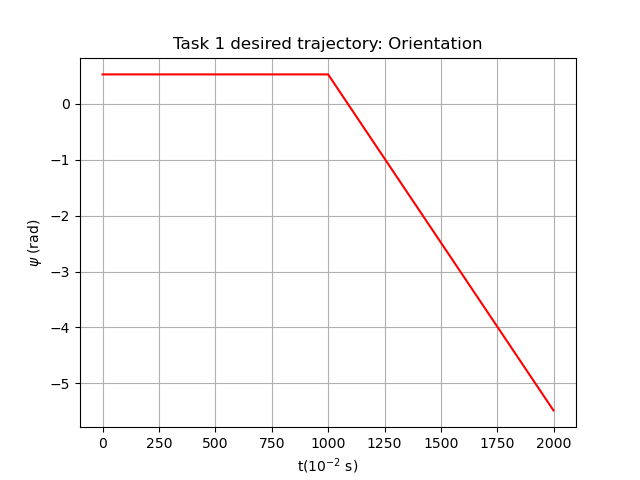
\includegraphics[width=\linewidth]{figs/despsi.png}
	\caption{Desired step $\psi$ trajectory}

	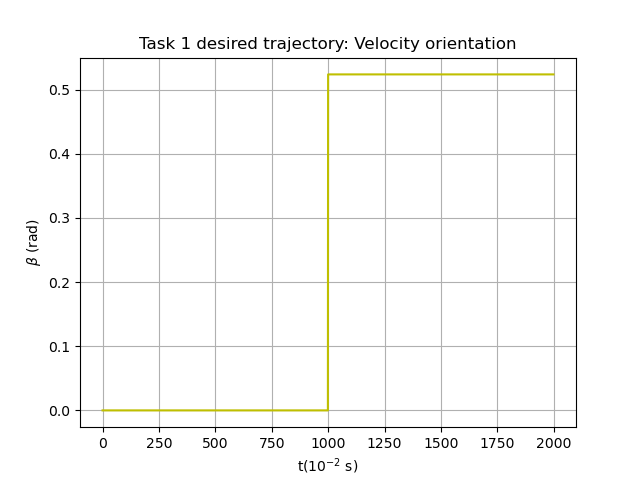
\includegraphics[width=\linewidth]{figs/desbeta.png}
	\caption{Desired step $\beta$ trajectory}
\end{figure} 

\begin{figure}[!h]
	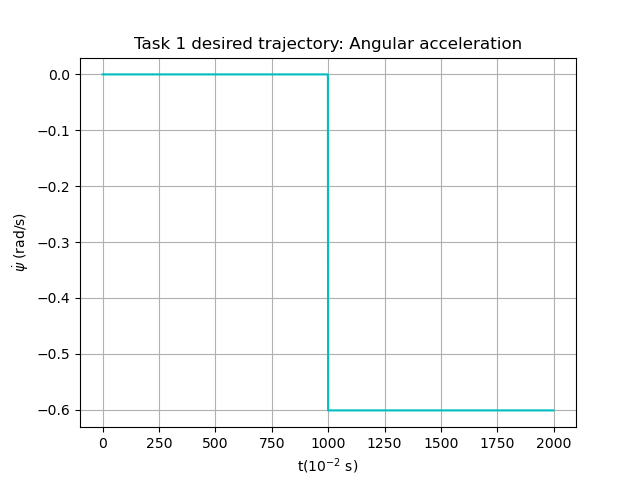
\includegraphics[width=\linewidth]{figs/despsid.png}
	\caption{Desired step $\dot{\psi}$ trajectory}
\end{figure} 

\FloatBarrier
\section{Optimal trajectory via Newton's algorithm}
To find an optimal trajectory between the two equilibria we will use a cost function that involves
the concept of quadratic form that allows us to input as parameters two weight matrices that represents how much
we want to track accurately a variable. The first weight matrix \texttt{QQt = 0.01*diag(0.1, 0.1, 100, 10, 100, 100)} 
is used for the state variables while the second one \texttt{RRt = 0.01*diag(5000, 0.00001)} is for the input variables.
\\This cost function will be minimized via a Newton's method, for the computation of the descent direction,
in which we can avoid to compute the Hessian of the dynamics by solving the costate equations and solving an affine linear quadratic problem;
and with a step size ($\gamma$) chosen by the Armijo's rule.
\\Additionally by using the shooting method we can further simplify the problem and consider it as unconstrained optimization problem with a 
single decision variable $u$.
\\To sum up the decision variable $u$ will be updated as:
\begin{align*}
	u_t^{k+1}=u_t^k+\gamma^k\Delta u_t^k\\
	x_t^{k+1}=f_t(x_t^{k+1},u_t^{k+1})
\end{align*}
The plots for which we need to pay more attention are the Armijo's one, in fact is possible to see if the algorithm is properly working,
if we are moving in the correct direction and if the step size chosen is the correct one or is outside of the admissible area between
the green and red lines. The following plots are taken every two iteration of the code.
\begin{figure}[!b]
	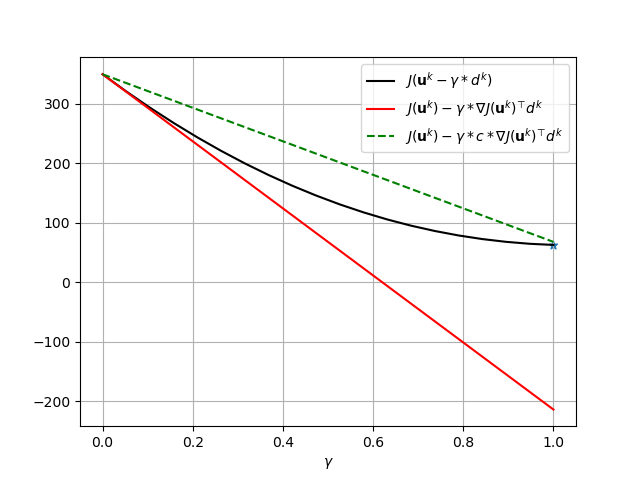
\includegraphics[width=0.5\columnwidth]{figs/Arm0.png}
	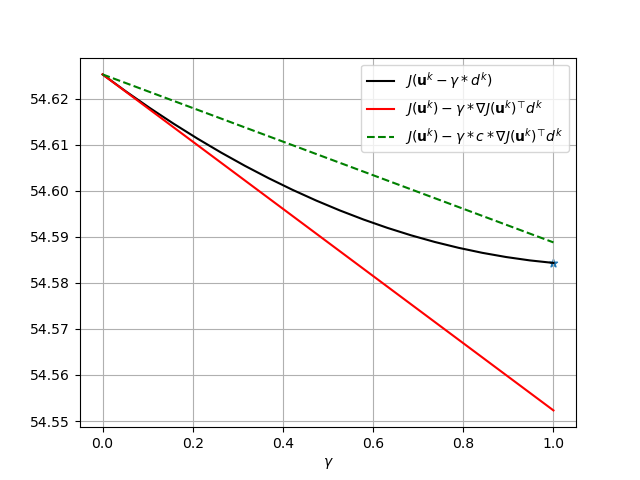
\includegraphics[width=0.5\columnwidth]{figs/arm2.png}
	\caption{Armijo's plot at the first and third iteration}
\end{figure}
\begin{figure}[ht]
	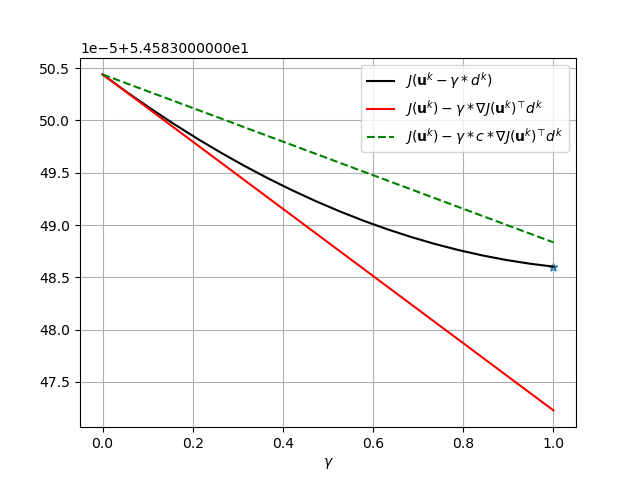
\includegraphics[width=0.5\linewidth]{figs/arm4.png}
    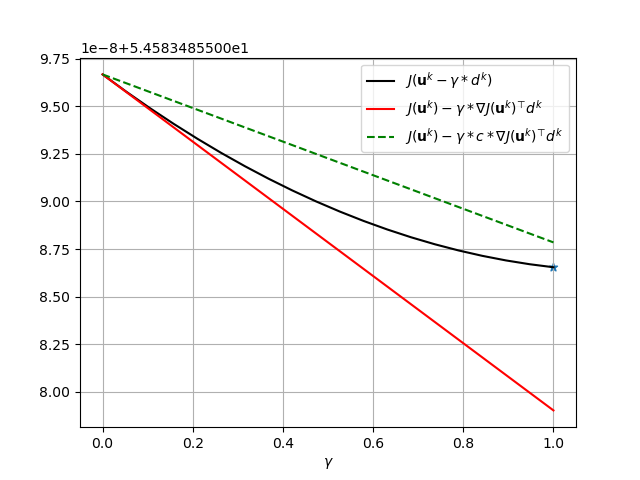
\includegraphics[width=0.5\linewidth]{figs/arm6.png}
	\caption{Armijo's plot at the fifth and seventh iteration}    
\end{figure} 

\begin{figure}[ht]
	\center
	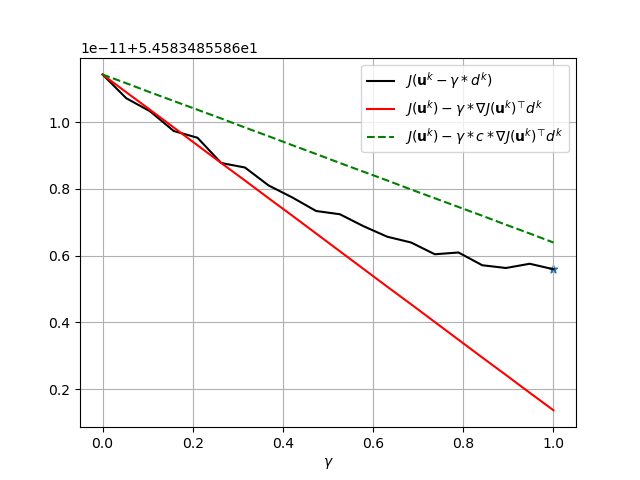
\includegraphics[width=0.75\linewidth]{figs/arm8.png}
	\caption{Armijo's plot at the last iteration}
	\label{fig:lastArm}
\end{figure} 

\FloatBarrier
As we can see from figure \ref{fig:lastArm} the algorithm is getting very close to the chosen sample period of the discretization and the result 
is that the curves are no longer so exact as in the first iterations so the central curve is no longer tangent to the red line.\\
In the following we can se the result of the applied methods on the obtained trajectories of the states and the inputs applied to the system.
\begin{figure}[htp]
    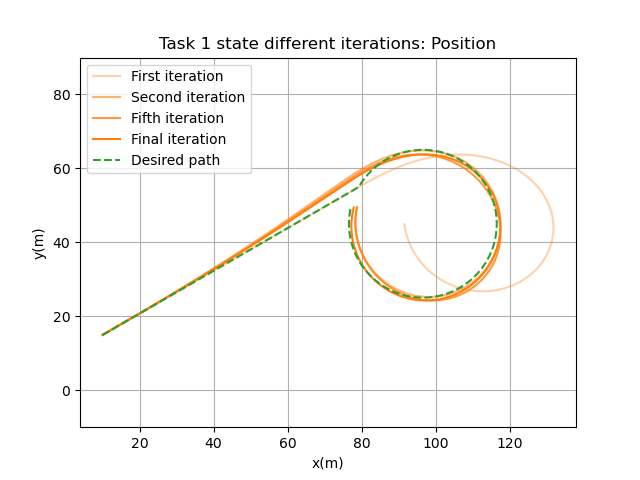
\includegraphics[width=0.5\textwidth]{figs/sometraj.png}
    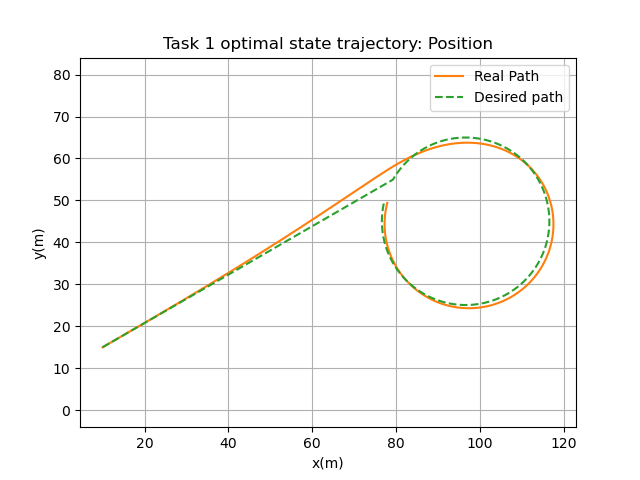
\includegraphics[width=0.5\textwidth]{figs/onetraj.png}
    \caption{Desired and obtained step position trajectory}
\end{figure}

\begin{figure}[htp]
    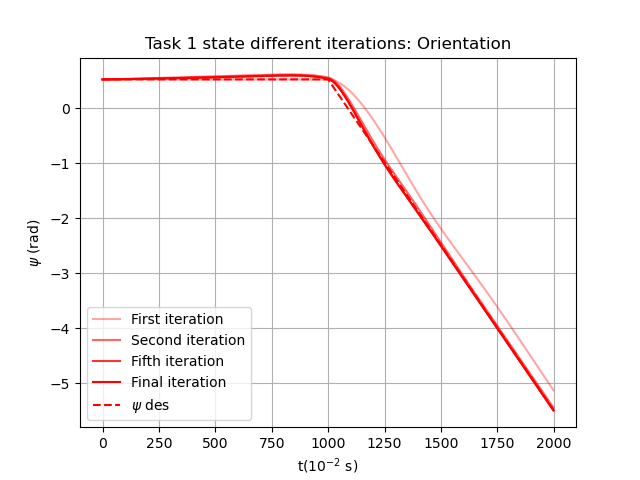
\includegraphics[width=0.5\textwidth]{figs/someorient.png}
    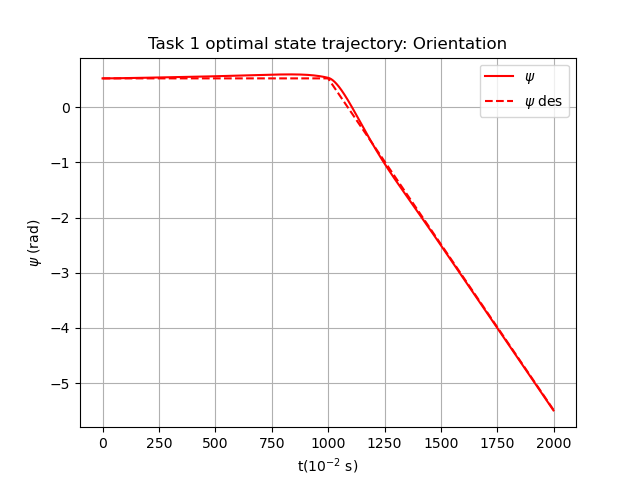
\includegraphics[width=0.5\textwidth]{figs/onepsi.png}
    \caption{Desired and obtained step orientation ($\psi$) trajectory}
\end{figure}

\begin{figure}[htp]
    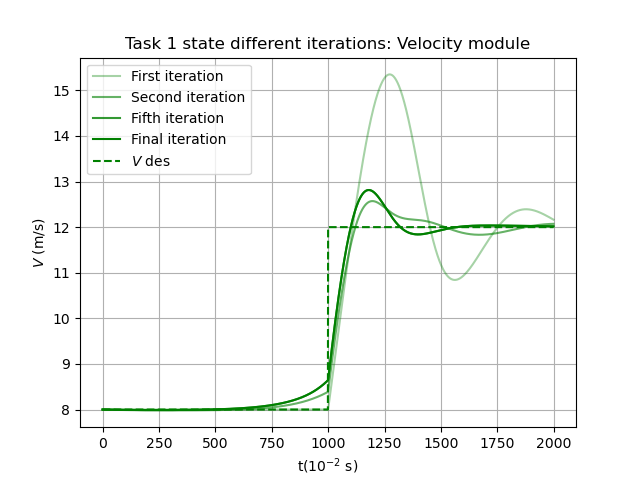
\includegraphics[width=0.5\textwidth]{figs/someV.png}
    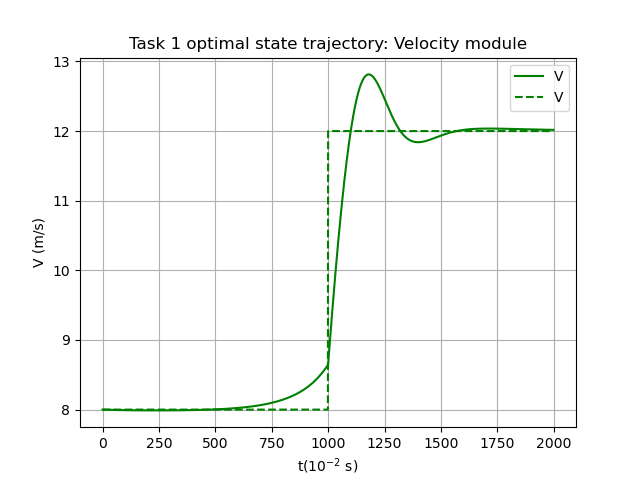
\includegraphics[width=0.5\textwidth]{figs/oneV.png}
    \caption{Desired and obtained step velocity trajectory}
\end{figure}

\begin{figure}[htp]
    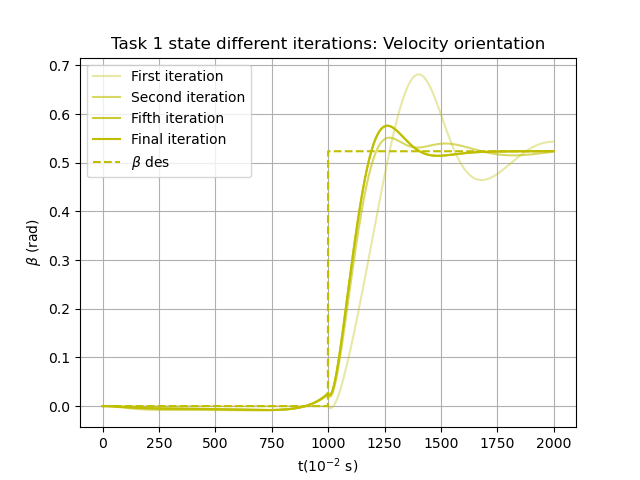
\includegraphics[width=0.5\textwidth]{figs/somebeta.png}
    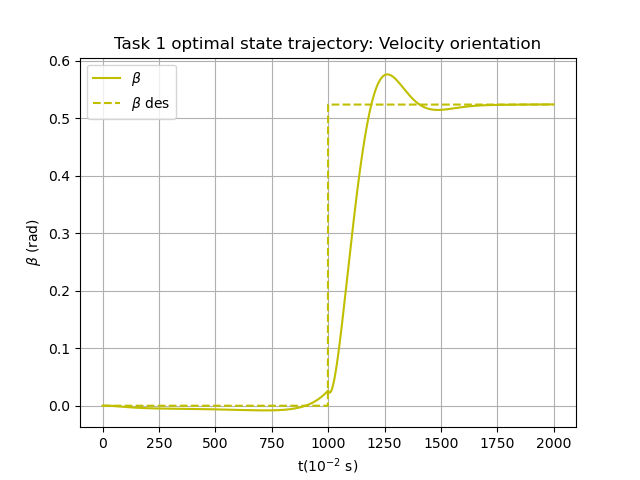
\includegraphics[width=0.5\textwidth]{figs/onebeta.png}
    \caption{Desired and obtained step $\beta$ trajectory}
\end{figure}

\begin{figure}[htp]
    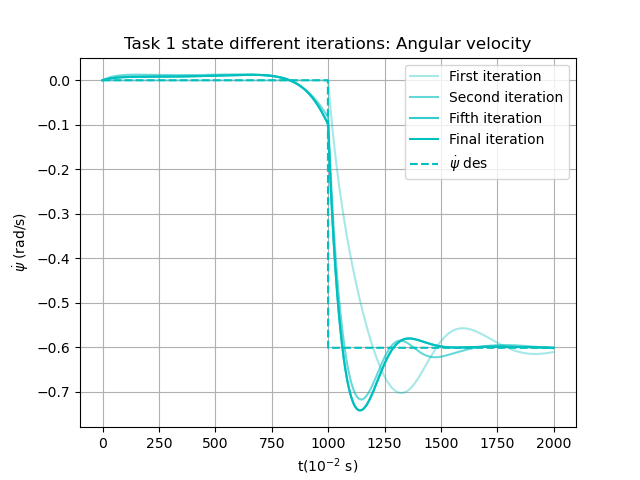
\includegraphics[width=0.5\textwidth]{figs/somepsid.png}
    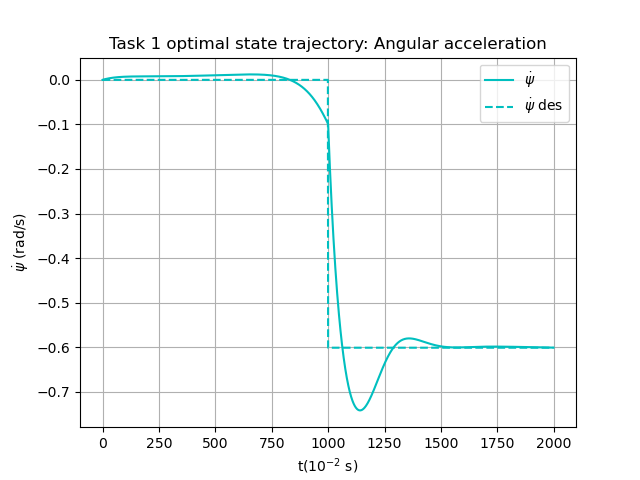
\includegraphics[width=0.5\textwidth]{figs/onepsid.png}
    \caption{Desired and obtained step $\dot{\psi}$ trajectory}
\end{figure}

\begin{figure}[htp]
    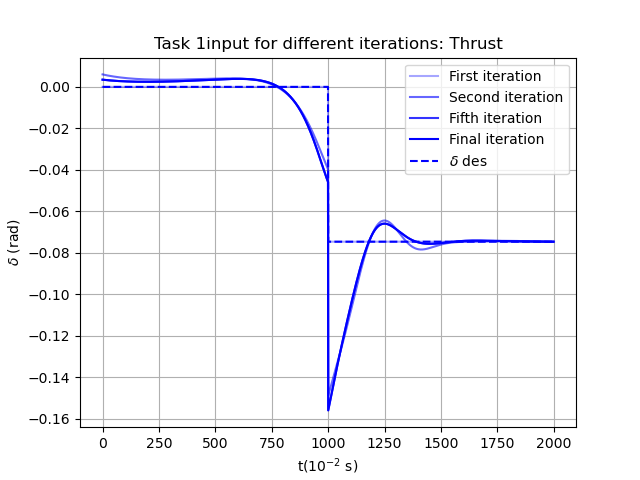
\includegraphics[width=0.5\textwidth]{figs/somedelta.png}
    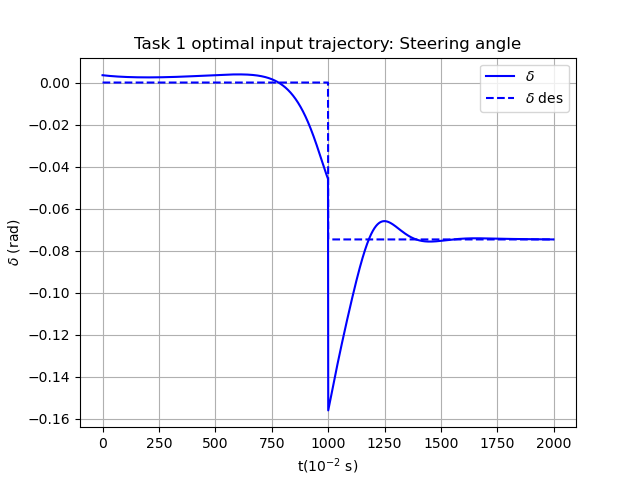
\includegraphics[width=0.5\textwidth]{figs/onedelta.png}
    \caption{Desired and obtained step $\delta$ trajectory}
	\label{fig:dstep}
\end{figure}

\begin{figure}[htp]
    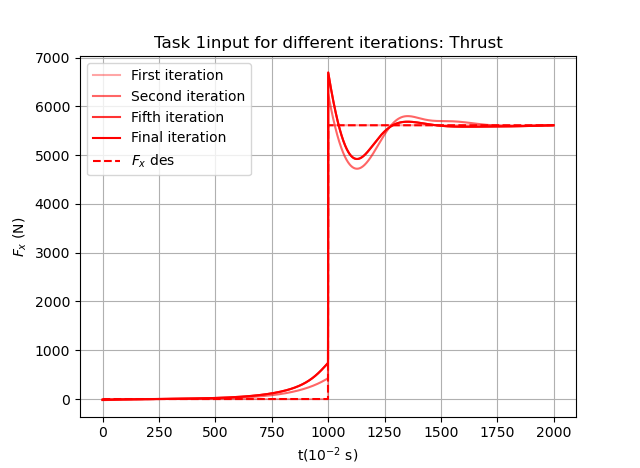
\includegraphics[width=0.5\textwidth]{figs/somefx.png}
    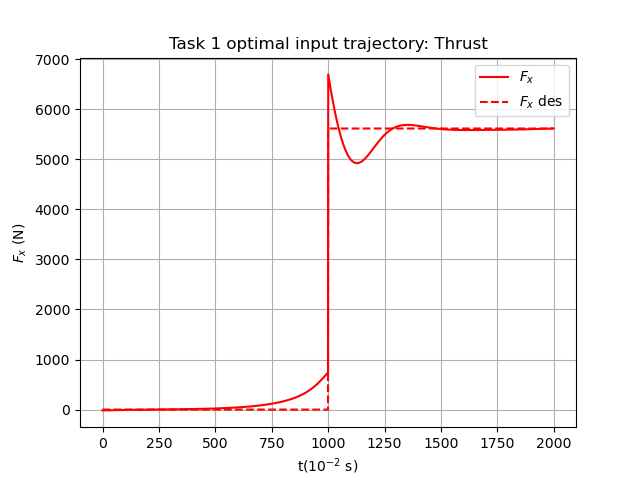
\includegraphics[width=0.5\textwidth]{figs/onefx.png}
    \caption{Desired and obtained step $F_x$ trajectory}
	\label{fig:fstep}
\end{figure}

\begin{figure}[htp]
    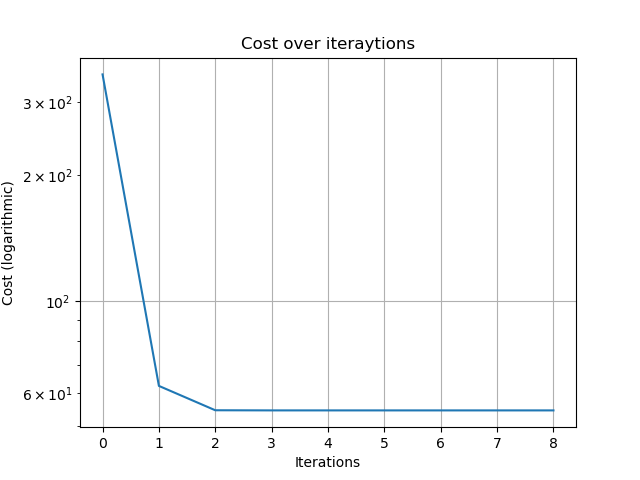
\includegraphics[width=0.5\textwidth]{figs/cost.png}
    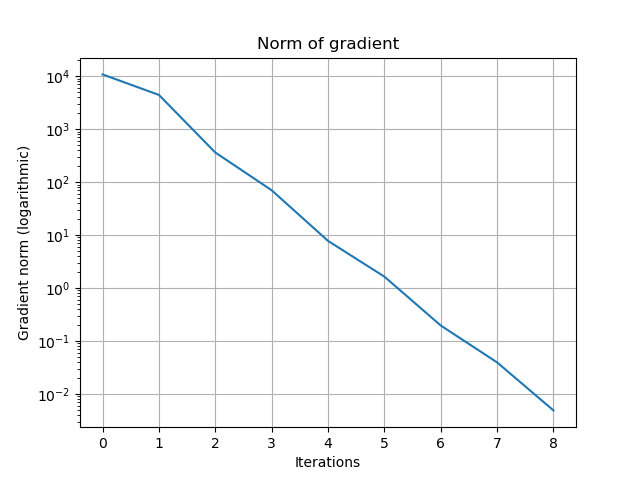
\includegraphics[width=0.5\textwidth]{figs/norm.png}
    \caption{Obtained decrease in cost function and norm of descent direction}
\end{figure}

\FloatBarrier
\section{Conclusions}
As we can see from figures \ref{fig:dstep} and \ref{fig:fstep} the request of a step change between the two equilibria
causes some overshoot in the control inputs in particular in $\delta$, however both the control inputs then stabilize at the desired values.
We found the values of the input cost matrix \texttt{RRt} to be extremely relevant: since the force $F_x$ is five orders of
magnitude greater than the other values, we had to take a very small penalty to that term in order to balance it.\\
We assumed this is due to the fact that the Newton's method uses a second order approximation and this outlier input value
could make the higher order terms more relevant in the computations.  
\chapter{Task 2 - Newton's method on smooth trajectory}
The second task required us to compute a smooth input state curve and find the optimal trajectory with respect to that. 
\section{Equilibrium computation and quasi-static pair}
The first choice to be made is which smooth curve to use to move between the two equilibrium values. In order to attain a smooth and at least twice derivable curve, namely $x(\cdot) \in \mathit{C}^2$, we decided to use a sigmoid. 
We tuned the parameters to make the curve symmetric with respect to the positive time interval, and to have a slower transition between the values. The desired curve we obtained for $\beta$ and $V$ ended up like:
\begin{equation}
	x(t)= x_{eq}^1  + (x_{eq}^2 - x_{eq}^1) \sigma(\frac{(t-\frac{T}{2})}{4T}) 
\end{equation}
We then obtain the desired curve for the restricted system by finding the quasi-static equilibrium pair for each of the points we found, as previously done in Task 1. This way we end up with the sigmoid desired curve for the velocities. In order to find the desired positions, we integrate them by using the velocities we just found. The final result can be found in figure:
\begin{figure}[!h]
	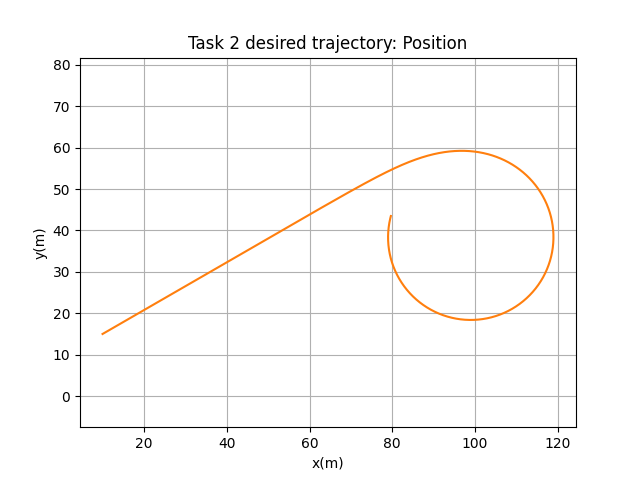
\includegraphics[width=\linewidth]{figs/des_pos_task2.png}
	\caption{Desired smooth position trajectory}
\end{figure} 

\begin{figure}[!h]
	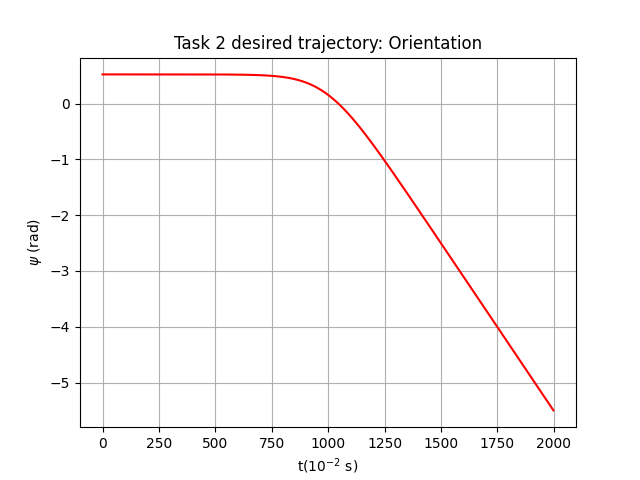
\includegraphics[width=\linewidth]{figs/des_or_task2.png}
	\caption{Desired smooth $\psi$ trajectory}

	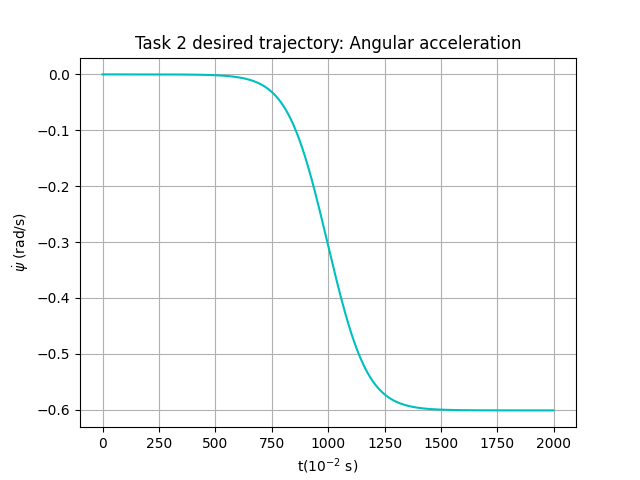
\includegraphics[width=\linewidth]{figs/des_psidot_task2.png}
	\caption{Desired smooth $\dot{\psi}$ trajectory}
	
\end{figure} 

\begin{figure}[!h]
	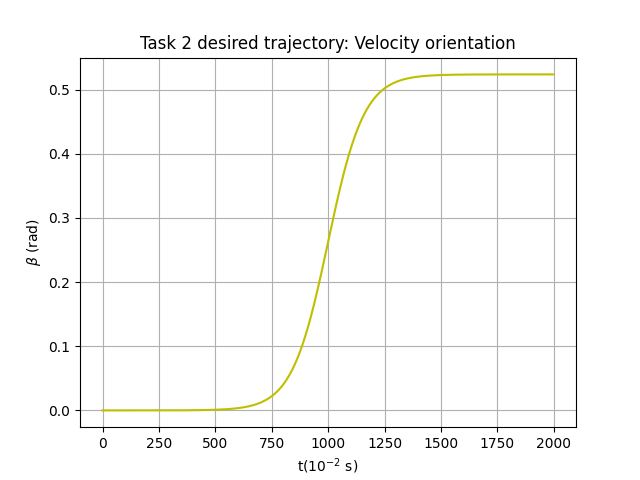
\includegraphics[width=\linewidth]{figs/des_beta_task2.png}
	\caption{Desired smooth $\beta$ trajectory}
	
	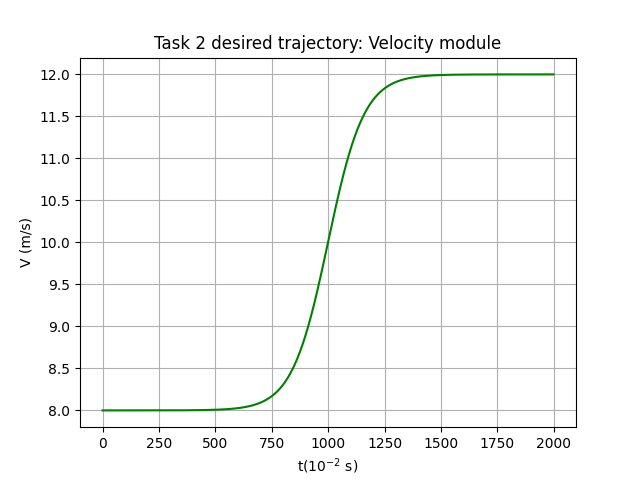
\includegraphics[width=\linewidth]{figs/des_V_task2.png}
	\caption{Desired smooth $V$ trajectory}
\end{figure} 

\FloatBarrier

\section{Newton's method on smooth curve}
We proceded with the Newton's method much in the same way we did for task one. We used the same cost matrices and applied the same routine. In figure the results at different iterations can be found. 

\begin{figure}[!h]
	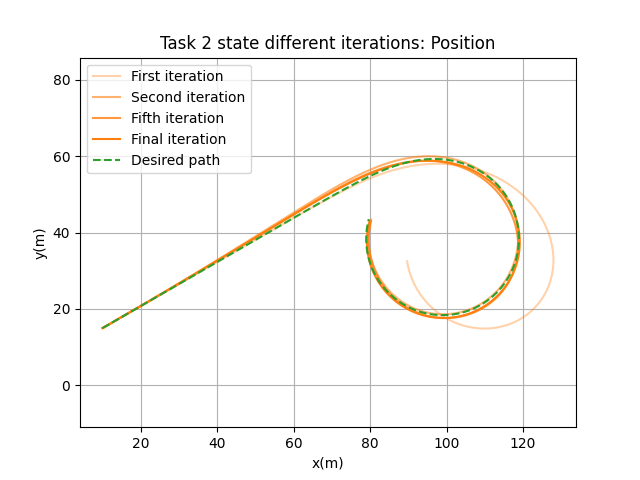
\includegraphics[width=0.5\columnwidth]{figs/positionsk_task2.png}
	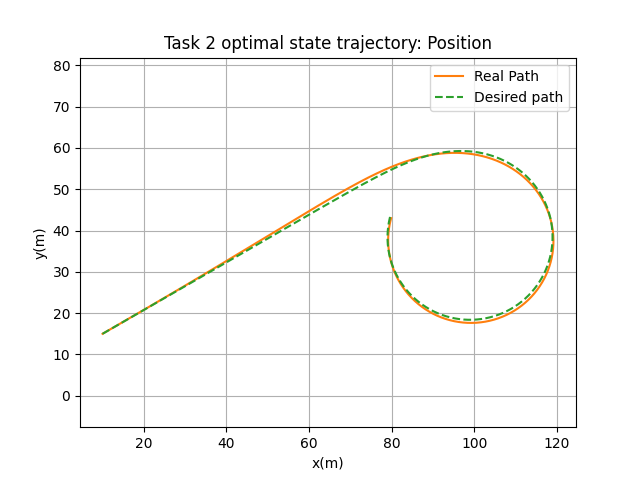
\includegraphics[width=0.5\columnwidth]{figs/onepos_task2.png}
	\caption{Desired smooth position trajectory}
\end{figure} 

\begin{figure}[!h]
	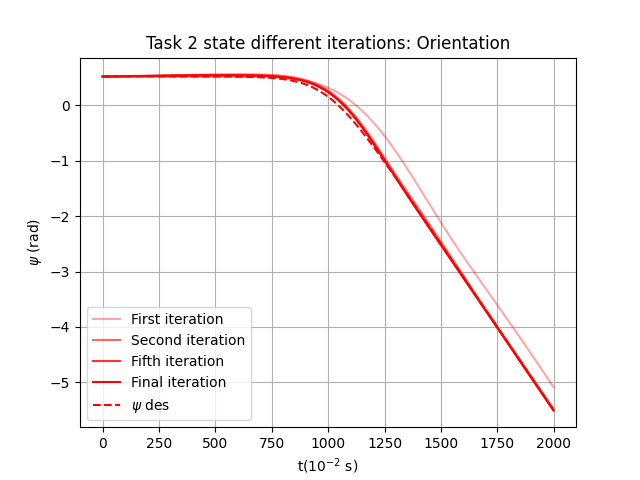
\includegraphics[width=0.5\columnwidth]{figs/orientationsk_task2.png}
	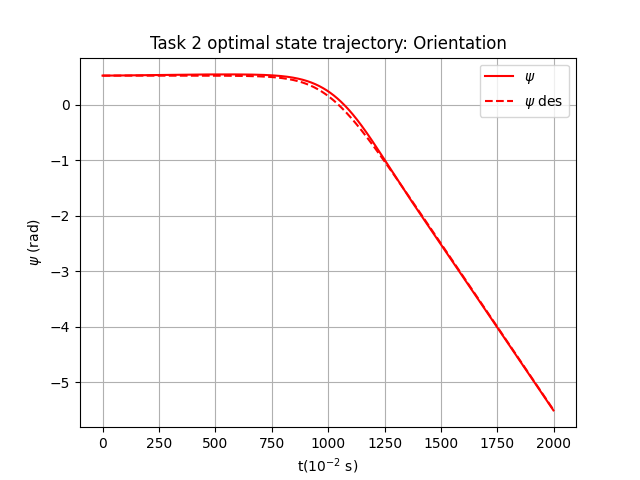
\includegraphics[width=0.5\columnwidth]{figs/oneor_task2.png}
	\caption{Desired smooth position trajectory}
\end{figure} 


\begin{figure}[!h]
	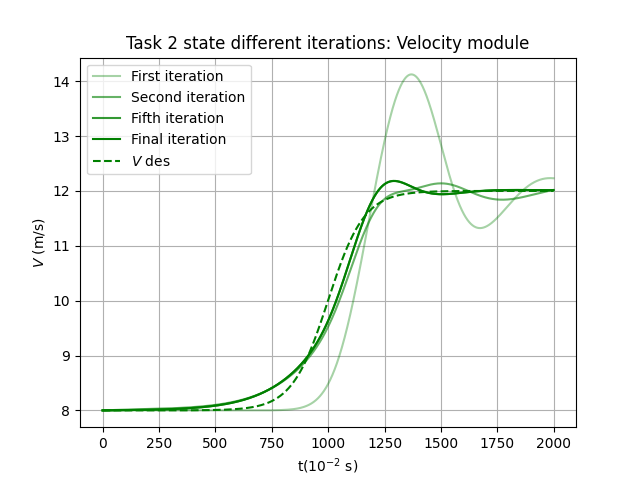
\includegraphics[width=0.5\columnwidth]{figs/velocitiesk_task2.png}
	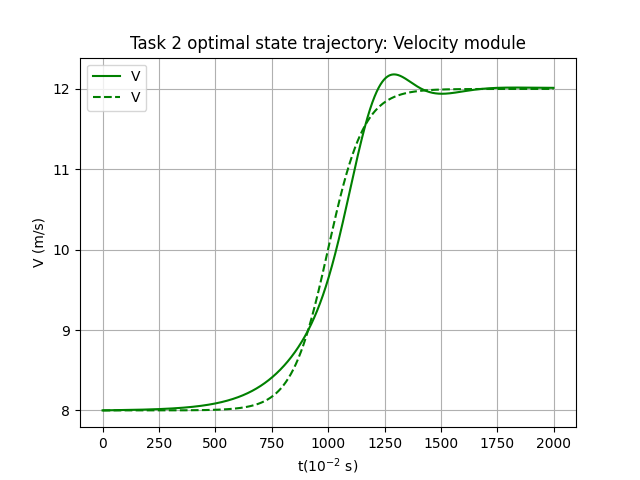
\includegraphics[width=0.5\columnwidth]{figs/oneV_task2.png}
	\caption{Desired smooth position trajectory}
\end{figure} 


\begin{figure}[!h]
	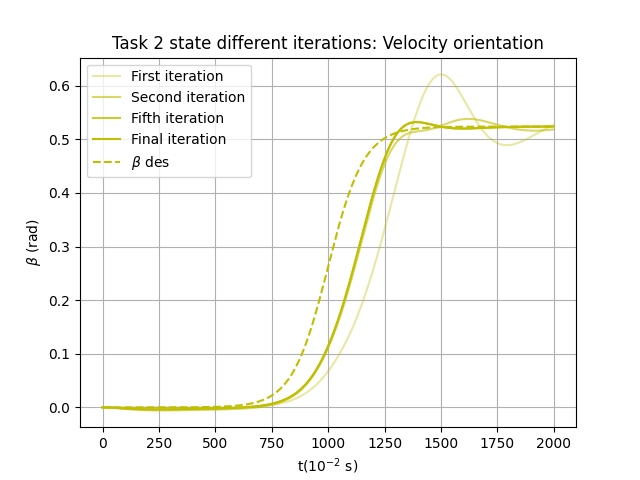
\includegraphics[width=0.5\columnwidth]{figs/betak_task2.png}
	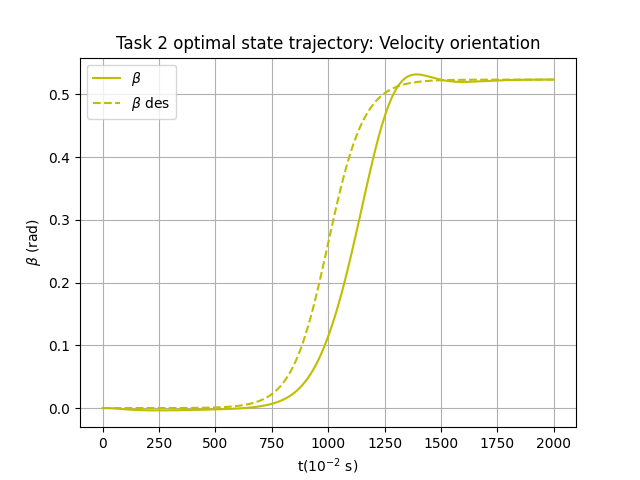
\includegraphics[width=0.5\columnwidth]{figs/onebeta_task2.png}
	\caption{Desired smooth position trajectory}
\end{figure} 


\begin{figure}[!h]
	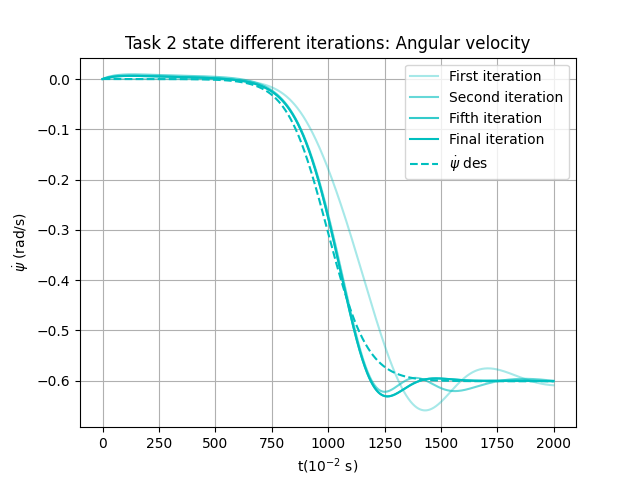
\includegraphics[width=0.5\columnwidth]{figs/psidotk_task2.png}
	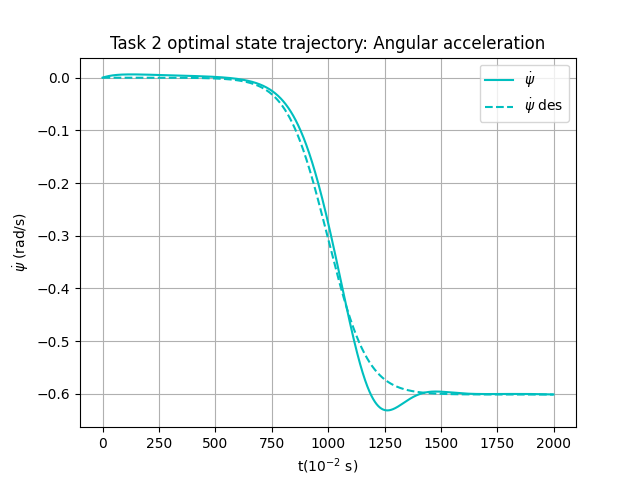
\includegraphics[width=0.5\columnwidth]{figs/onepsidot_task2.png}
	\caption{Desired smooth position trajectory}
\end{figure} 


\begin{figure}[!h]
	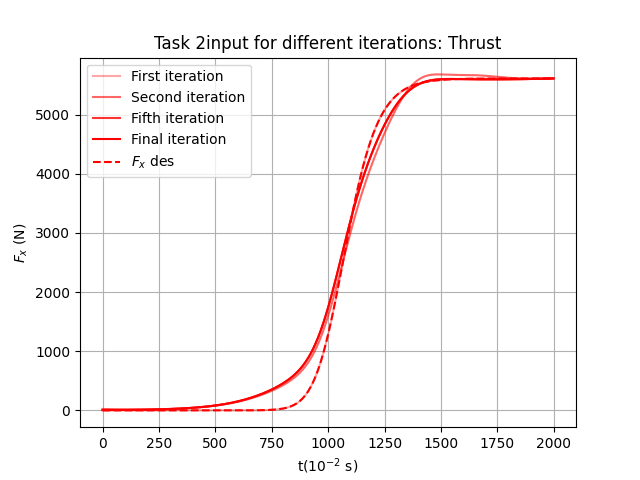
\includegraphics[width=0.5\columnwidth]{figs/Fxk_task2.png}
	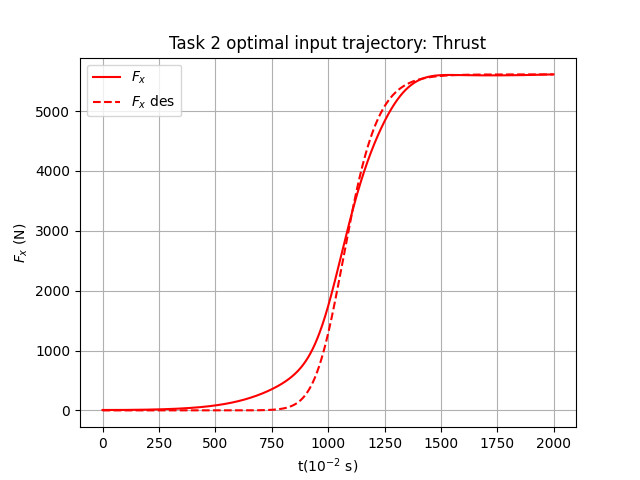
\includegraphics[width=0.5\columnwidth]{figs/Onefx_task2.png}
	\caption{Desired smooth position trajectory}
\end{figure} 


\begin{figure}[!h]
	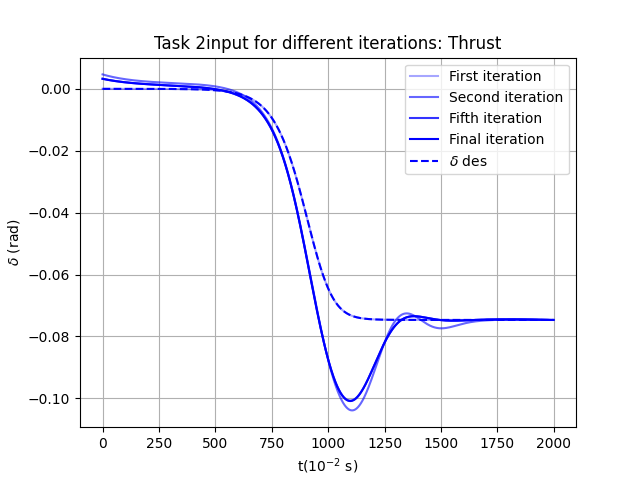
\includegraphics[width=0.5\columnwidth]{figs/deltak_task2.png}
	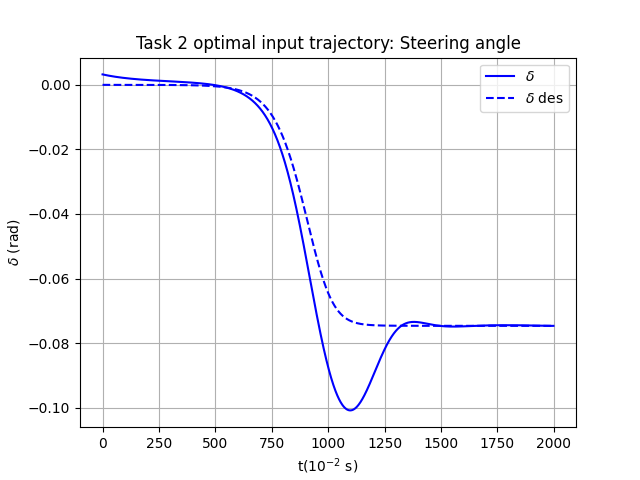
\includegraphics[width=0.5\columnwidth]{figs/onedelta_task2.png}
	\caption{Desired smooth position trajectory}
\end{figure} 


\FloatBarrier

Below are some of the Armijo's plots for the secon task. The plot was taken every two iterations.
\begin{figure}[!h]
	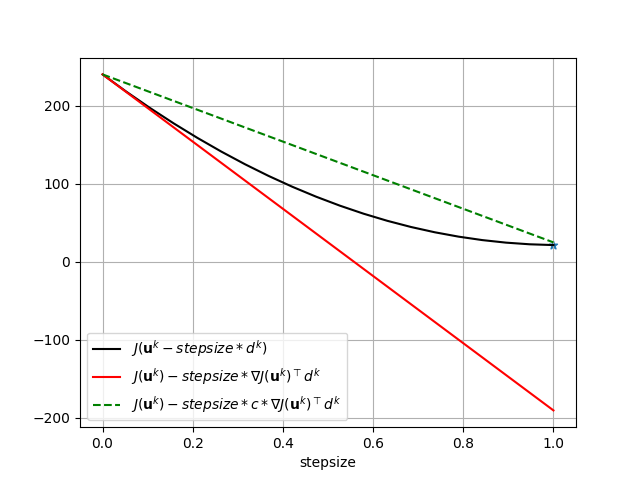
\includegraphics[width=0.5\linewidth]{figs/arm0_task2.png}
	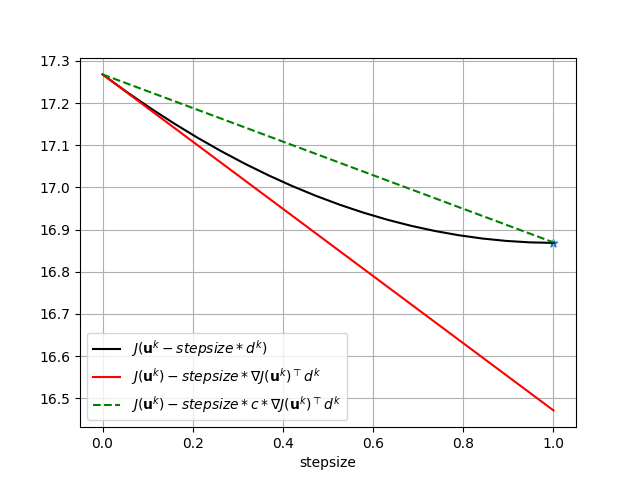
\includegraphics[width=0.5\linewidth]{figs/arm2_task2.png}
	\caption{Armijo's plot at first and third iteration}
\end{figure}
\begin{figure}[!h]
	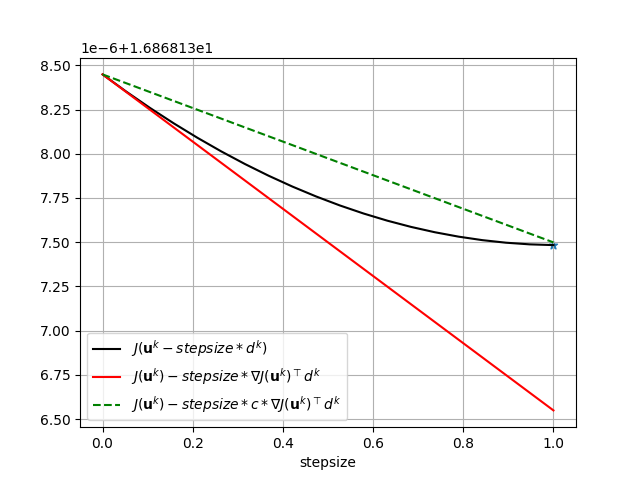
\includegraphics[width=0.5\linewidth]{figs/arm4_task2.png}
	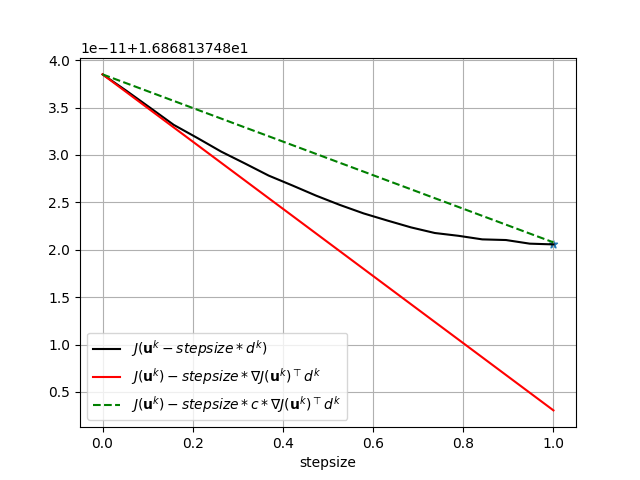
\includegraphics[width=0.5\linewidth]{figs/arm6_task2.png}
	\caption{Armijo's plot at the fifth and last iteration}
\end{figure} 

\FloatBarrier

Lastly, the plots for the cost and gradient norm over iterations can be found here.
\begin{figure}[!h]
	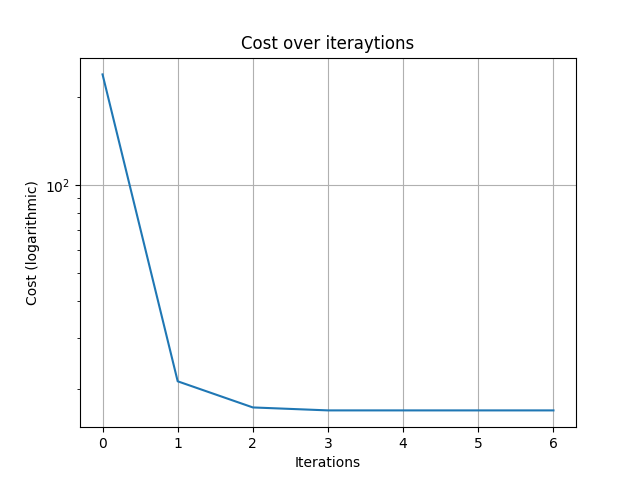
\includegraphics[width=0.5\linewidth]{figs/cost_iter_task2.png}
	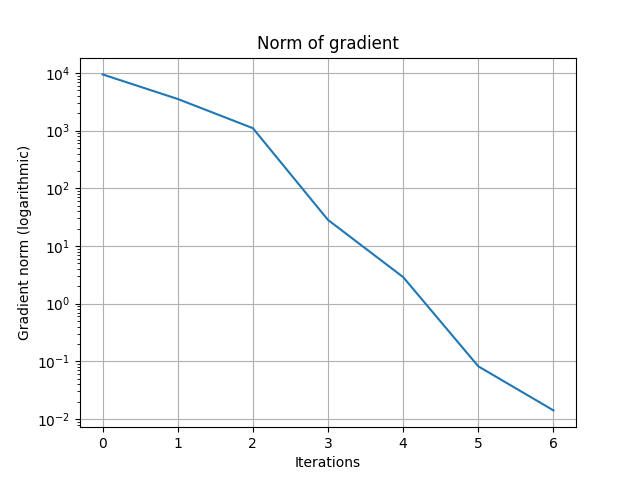
\includegraphics[width=0.5\linewidth]{figs/gradientnorm_task2.png}
	\caption{Armijo's plot at the fifth and last iteration}
\end{figure} 

\section{Conclusions}
The smooth desired curve leads to a nicer trajectory in terms of overshooting and use of the inputs. The overall cost of the trajectory is $16,87$, which is less then a third of the cost for the step trajectory ($54,58$). The inputs don't have discontinuities anymore and, as seen in the plots, stay closer to the desired curve (the quasi-static input curve)than in task one. Overall, we can clearly see the advantage in asking for a smooth input state curve rather than a step. 
\chapter{Task 3 - Trajectory tracking via LQR}
In this task the objective is to design a linear quadratic regulator [LQR] able to follow the smooth optimal trajectory generated in the 
previous task.

\section{Problem setup}
The first step needed to achieve our goal is to linearize the system dynamics, computed in Task 0, about the smooth optimal trajectory $(x^{opt},u^{opt})$,
obtained in Task 2, in order to obtain $A^{opt}$ and $B^{opt}$. Then the idea is to use a regulator that will reject disturbances, and will try to follow the 
optimal trajectory. To do that, we have to solve a Linear quadratic optimization problem, with a quadratic cost function, in which the cost matrices were a degree of freedom,
and the linearized dynamics over the optimal trajectory.

\section{Parameters and results}
Running some simulation, we found great results using as matrices $Q^{reg}$ and $R^{reg}$ the same matrices used in the cost function for the Newton's method.
To test the performances of our regulator, we will inject in the system some random error (5-10-20\% of the maximum value reached during the trajectory for each state)
in the initial conditions.
\\Then we need to solve the LQ optimal control problem to find the feedback gain matrix $K_t^{reg}$ needed to update $u$ bye the equation: 
\begin{center}
    $u_t=u_t^{opt}+K_t^{reg}(x_t-x_t^{opt})$\\
    $x_{t+1}=f_t(x_t,u_t)$
\end{center}

In the following plots we can see the tracking performances of the LQR algorithm used.
\begin{figure}[!h]
    \center
	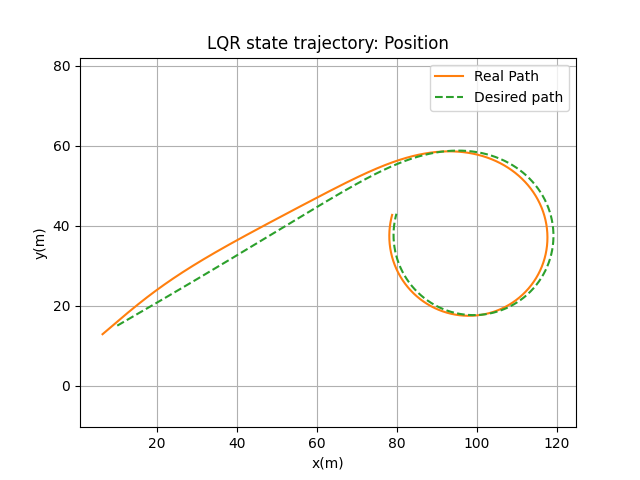
\includegraphics[height=70mm]{figs/_lqr_xy_5.png}	
	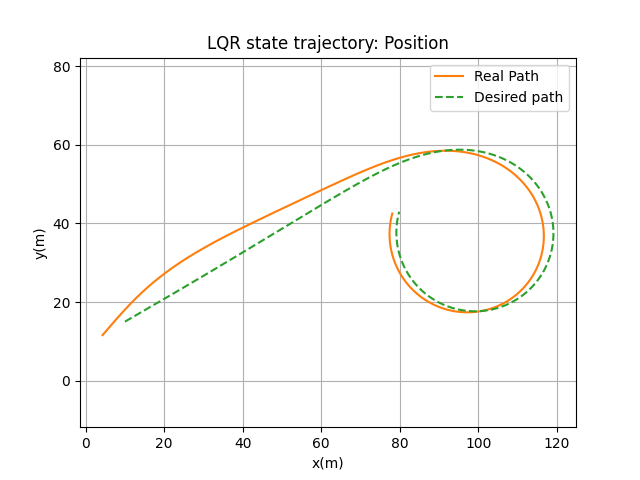
\includegraphics[height=70mm]{figs/_lqr_xy_10.png}	
    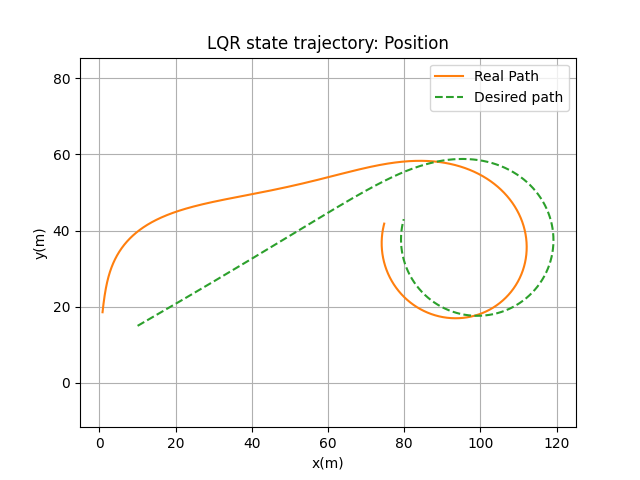
\includegraphics[height=70mm]{figs/_lqr_xy_20.png}	
	\caption{Tracked position trajectory with 5-10-20\% relative error on $x_0$}
\end{figure} 

\begin{figure}[!h]
    \center
	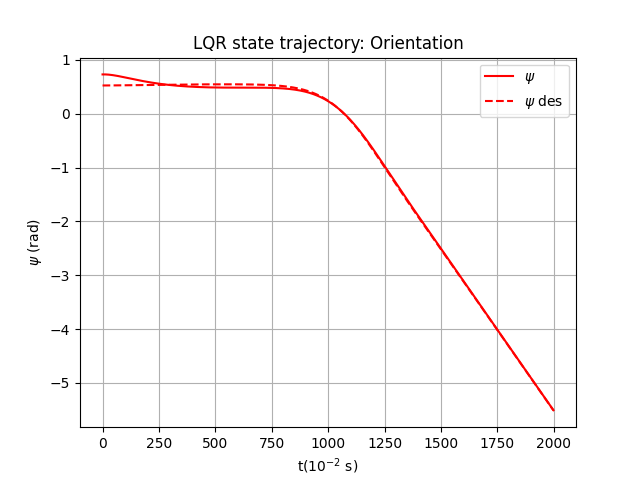
\includegraphics[height=70mm]{figs/_lqr_psi_5.png}	
	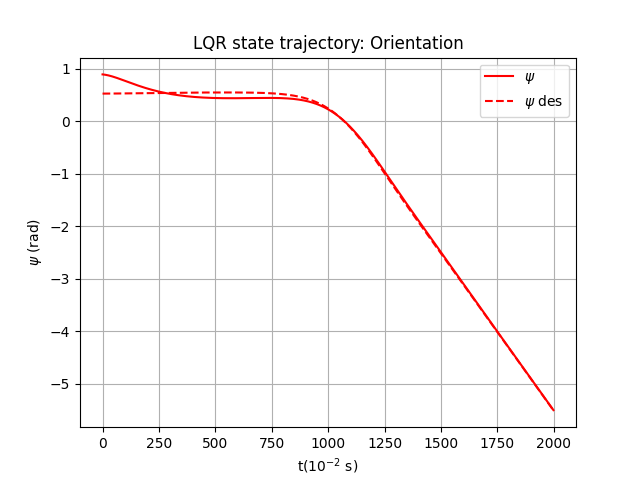
\includegraphics[height=70mm]{figs/_lqr_psi_10.png}	
    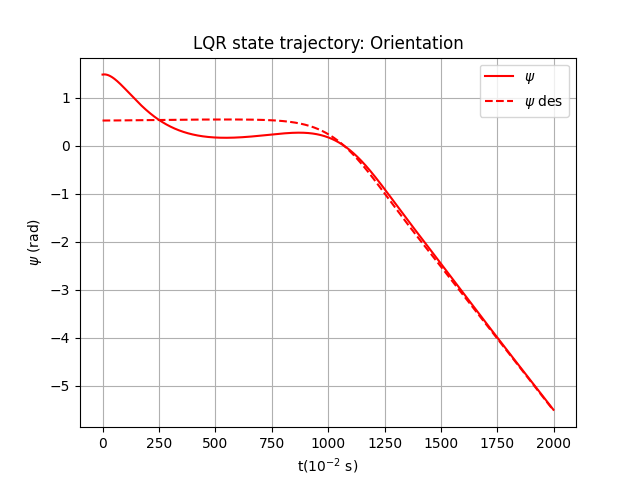
\includegraphics[height=70mm]{figs/_lqr_psi_20.png}	
	\caption{Tracked $\psi$ trajectory with 5-10-20\% relative error on $x_0$}
\end{figure} 

\begin{figure}[!h]
    \center
	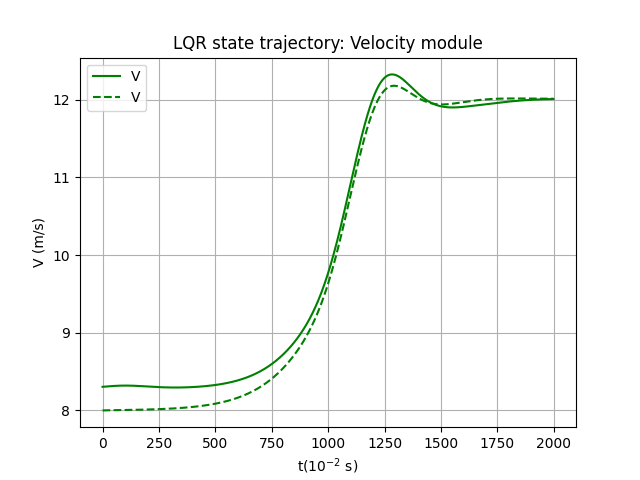
\includegraphics[height=70mm]{figs/_lqr_V_5.png}	
	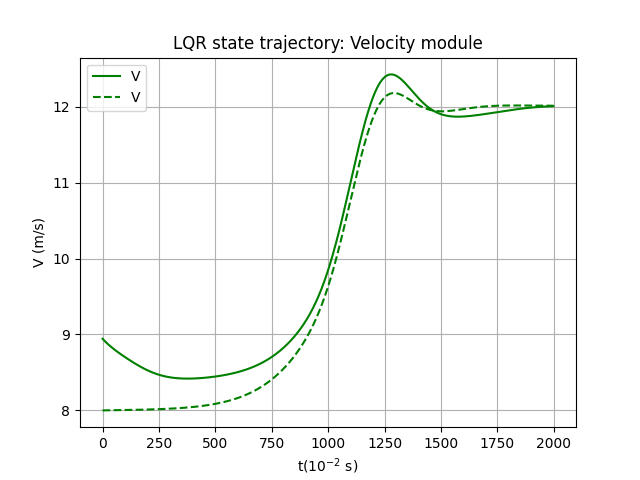
\includegraphics[height=70mm]{figs/_lqr_V_10.png}	
    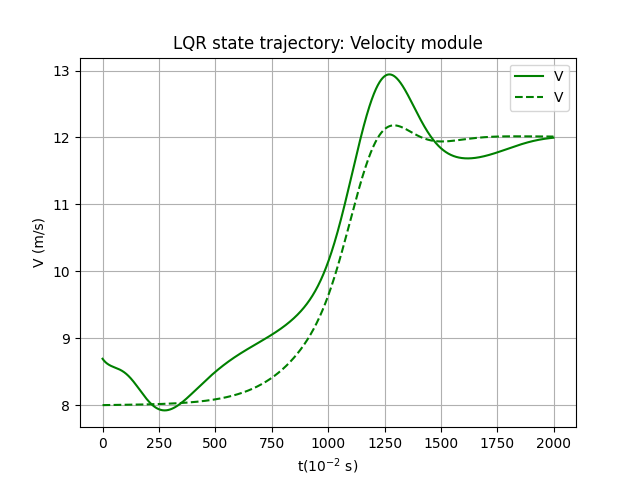
\includegraphics[height=70mm]{figs/_lqr_V_20.png}	
	\caption{Tracked $V$ trajectory with 5-10-20\% relative error on $x_0$}
\end{figure} 

\begin{figure}[!h]
    \center
	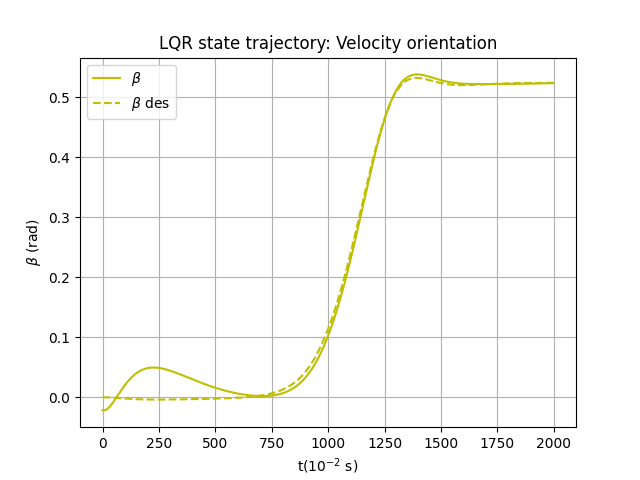
\includegraphics[height=70mm]{figs/_lqr_beta_5.png}	
	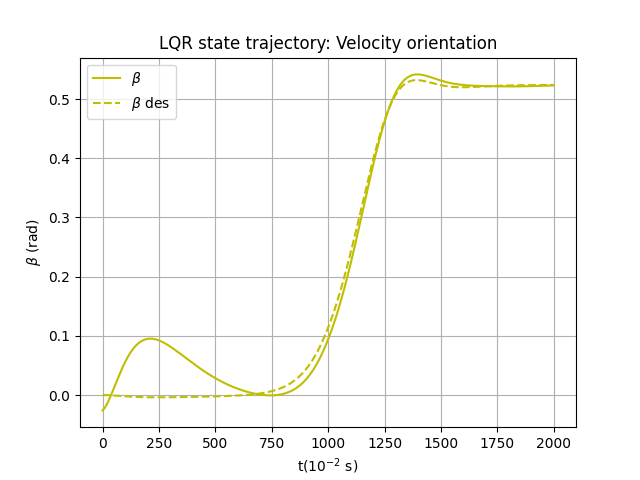
\includegraphics[height=70mm]{figs/_lqr_beta_10.png}	
    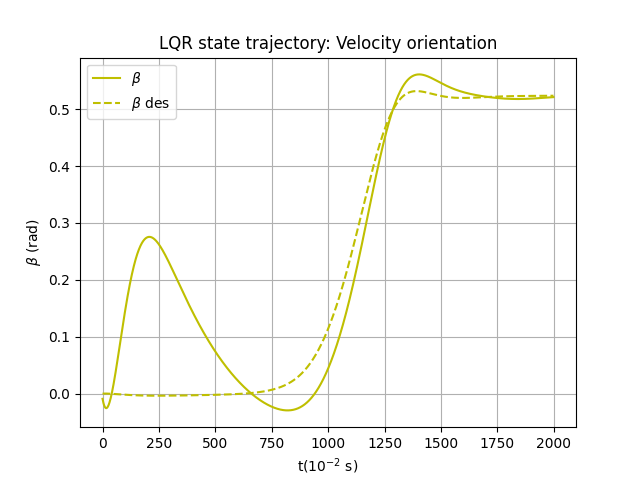
\includegraphics[height=70mm]{figs/_lqr_beta_20.png}	
	\caption{Tracked $\beta$ trajectory with 5-10-20\% relative error on $x_0$}
\end{figure} 

\begin{figure}[!h]
    \center
	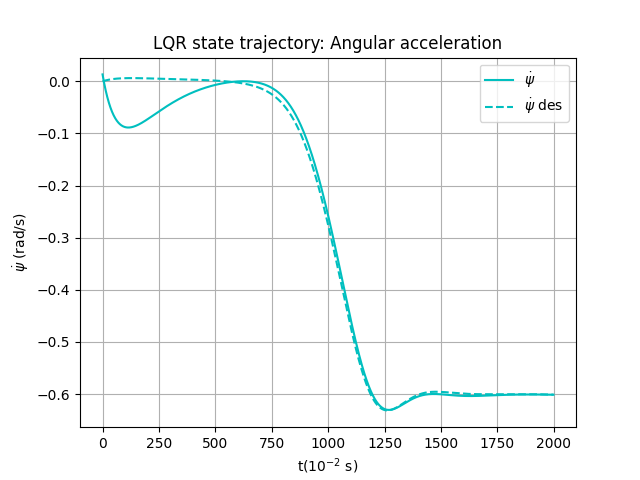
\includegraphics[height=70mm]{figs/_lqr_psidot_5.png}	
	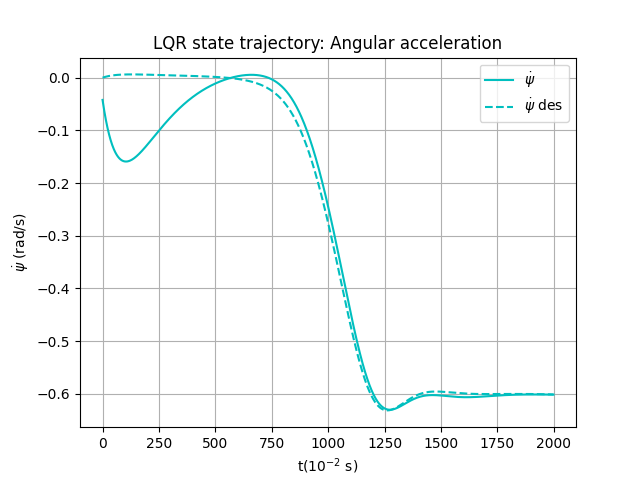
\includegraphics[height=70mm]{figs/_lqr_psidot_10.png}	
    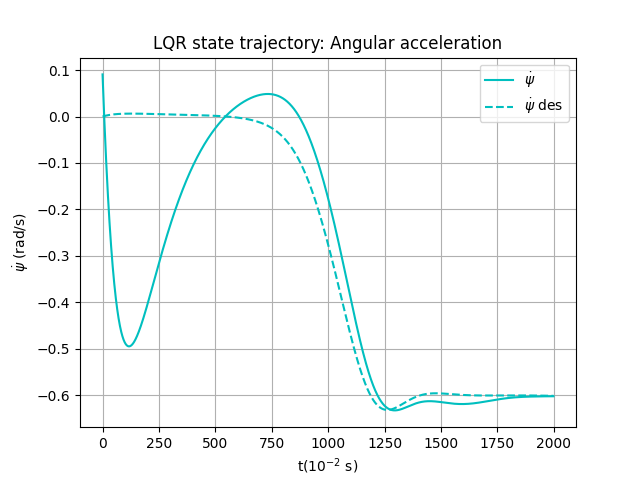
\includegraphics[height=70mm]{figs/_lqr_psidot_20.png}	
	\caption{Tracked $\dot{\psi}$ trajectory with 5-10-20\% relative error on $x_0$}
\end{figure} 

\begin{figure}[!h]
    \center
	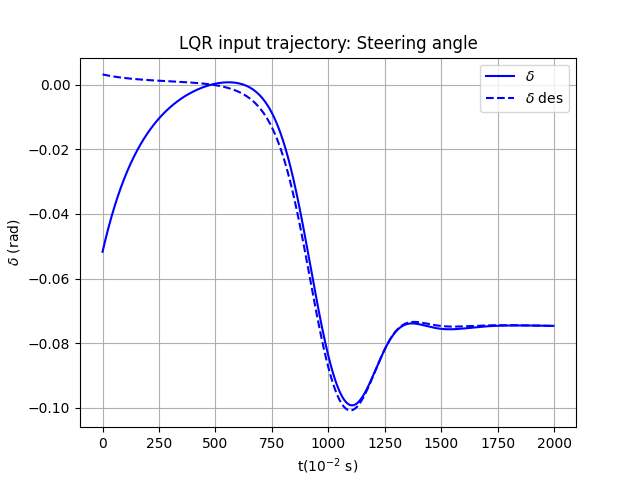
\includegraphics[height=70mm]{figs/_lqr_delta_5.png}	
	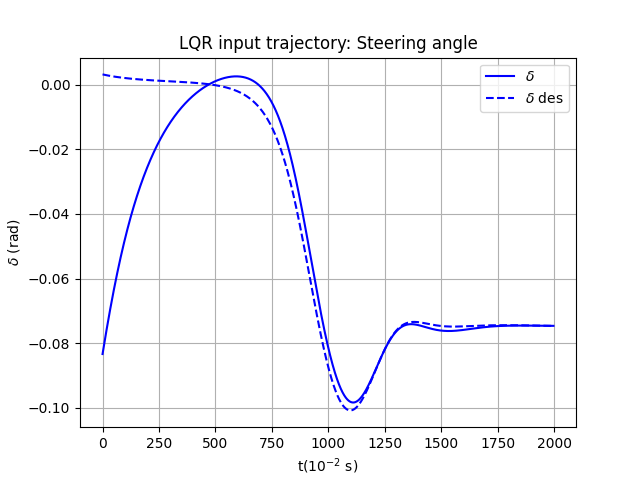
\includegraphics[height=70mm]{figs/_lqr_delta_10.png}	
    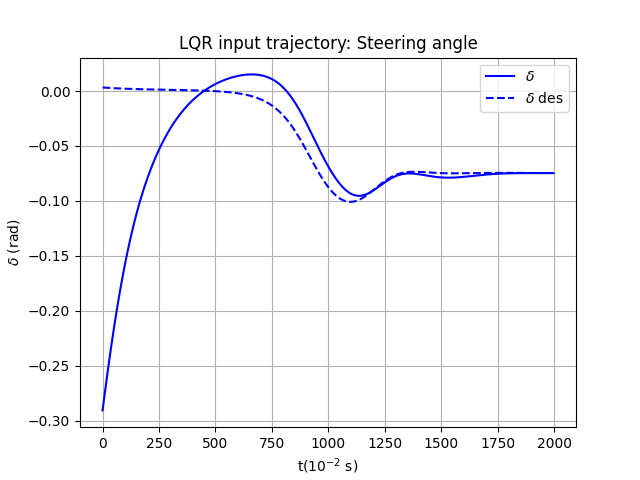
\includegraphics[height=70mm]{figs/_lqr_delta_20.png}	
	\caption{Tracked $\delta$ trajectory with 5-10-20\% relative error on $x_0$}
\end{figure} 

\begin{figure}[!h]
    \center
	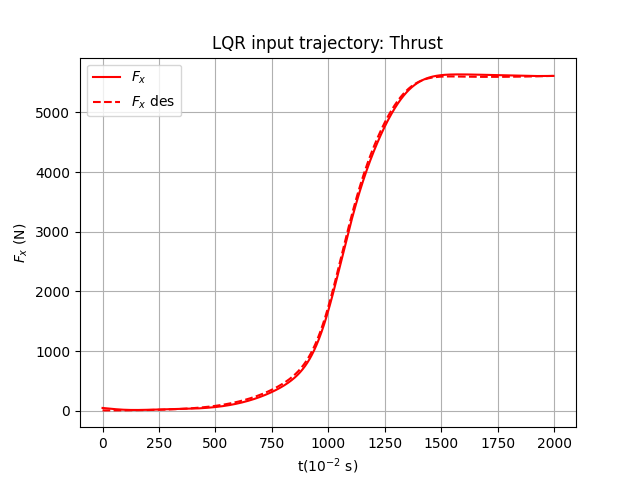
\includegraphics[height=70mm]{figs/_lqr_Fx_5.png}	
	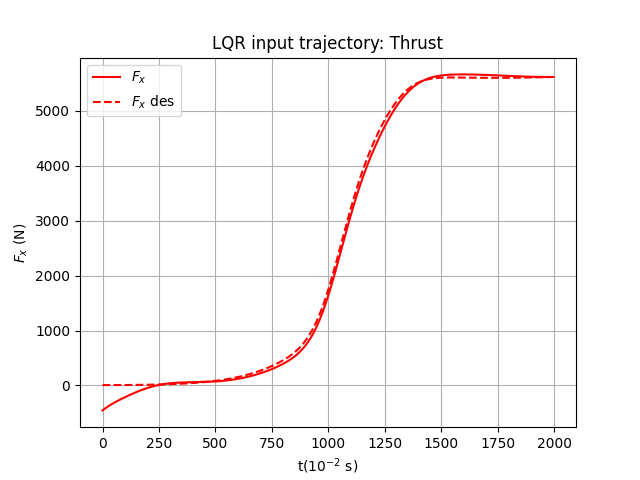
\includegraphics[height=70mm]{figs/_lqr_Fx_10.png}	
    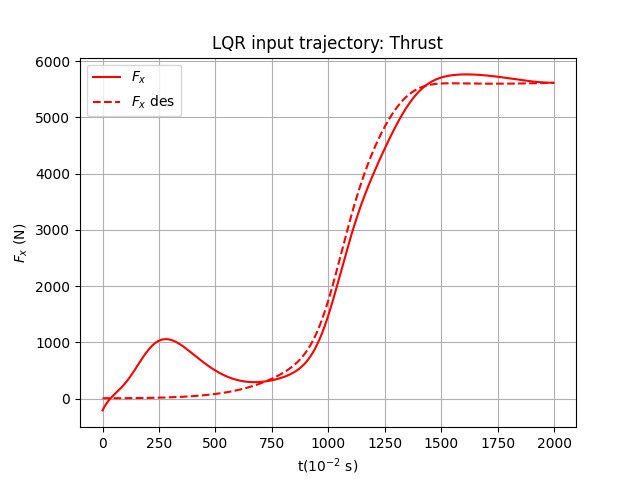
\includegraphics[height=70mm]{figs/_lqr_Fx_20.png}	
	\caption{Tracked $F_x$ trajectory with 5-10-20\% relative error on $x_0$}
\end{figure} 

\FloatBarrier
\section{Conclusions}
The LQR algorithm proved to be very robust with respect to initial condition error, 
indeed all the state variables with 5\% and 10\% error were accurately tracked and
only the trajectory with 20\% error reached the desired velocity bringing the system
in a steady state with some offset in the final position. 
\chapter{Task 4 - Trajectory tracking via MPC}
The goal of this task was to control the system around the optimal trajectory found in task 2 by means of Model Predictive control (hereafter referred as MPC).
\section{Problem setup}
In order to set up an MPC controller, the first step is to linearize around the desired trajectory. This way, we are able to use the \texttt{cvxpy} library to solve the problem quickly, by also taking into account possible path constraints on the input or the state.
We designed the function \texttt{linear\_ mpc} specifically to handle this task. At each time instant, we run the optimization problem on a time window of \texttt{$T_{mpc}$} and use the first input of the sequence. For plotting purposes we keep track of all the inputs we give to the system. 

\section{Parameters}
Even if we were able to tune the cost parameters $Q_{reg}$ and $R_{reg}$ as a degree of freedom, after running some experiments we found the same values we used in the optimization problem to be optimal. 
We implemented a random noise to be added. We tried to evaluate the system evolution for error on one individual component per experiments and the tracking was almost completely matching. However, for lack of space, these results won't be added in this report. 
We tried to evaluate the evolution of the system with the initial condition $x_0$ subject to a random error proportional to the maximum aplitude of each component, namely
\begin{equation}
 	x_{0,i}^{real}=x_{0,i}^{opt} \pm max_t(x_i^{opt})*p*randn, i \in 1,...,n
\end{equation}
with $p$ desired percentage, and $randn$ random number such that $-0.5<randn<0.5$. 
\section{Results}
Below are the plots for the results for $p$ varying from $10$ to $40$.

\begin{figure}[!h]
    \center
	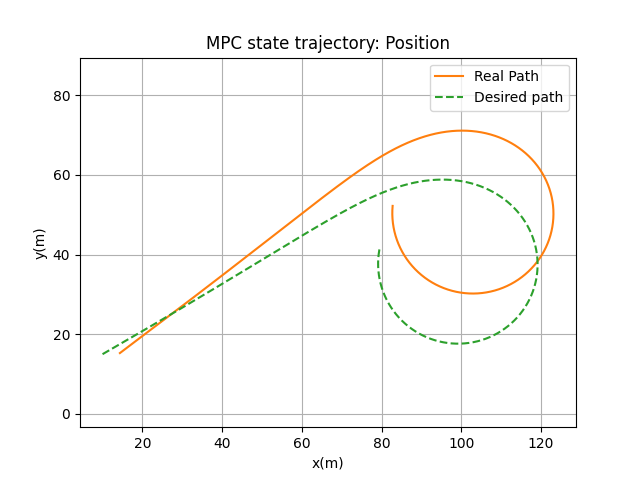
\includegraphics[height=70mm]{figs/_mpc_xy_5.png}	
	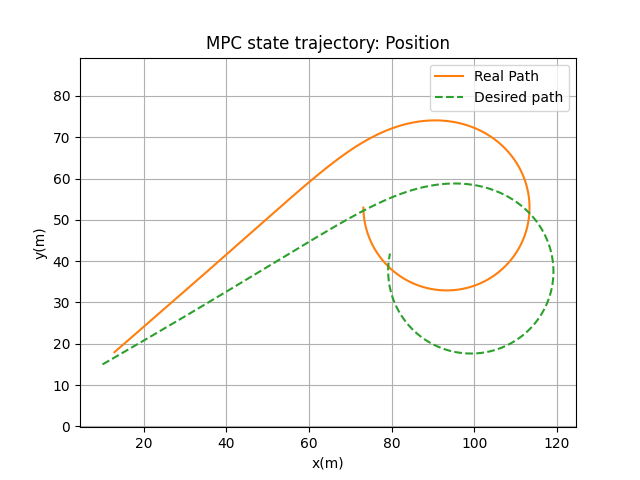
\includegraphics[height=70mm]{figs/_mpc_xy_10.png}	
    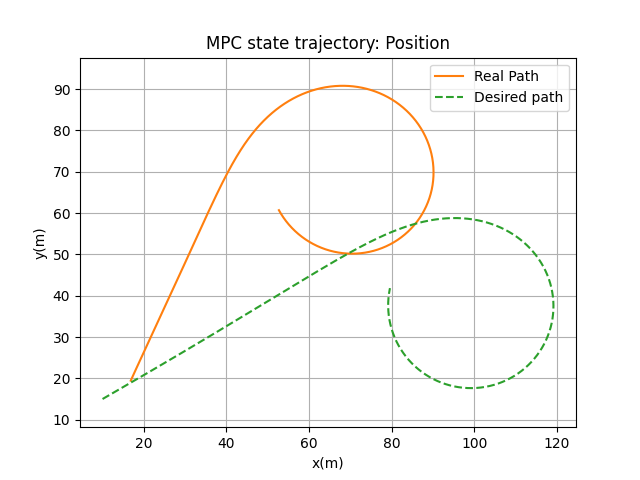
\includegraphics[height=70mm]{figs/_mpc_xy_20.png}	
	\caption{Tracked position trajectory with 5-10-20\% relative error on $x_0$}
\end{figure} 

\begin{figure}[!h]
    \center
	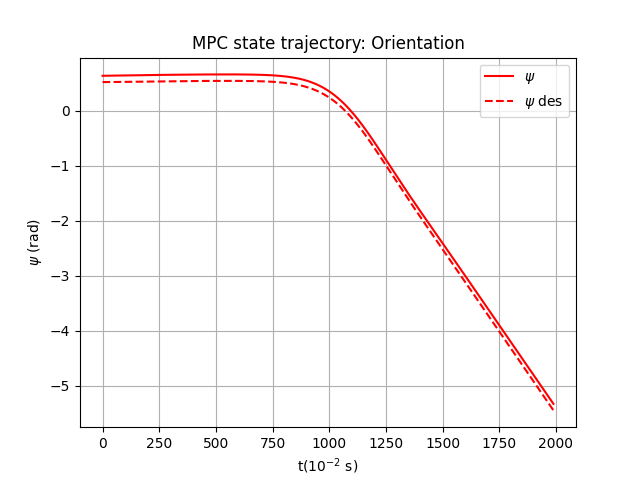
\includegraphics[height=70mm]{figs/_mpc_psi_5.png}	
	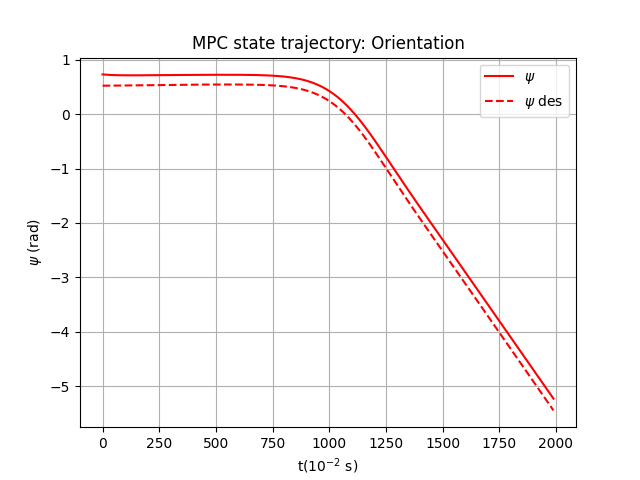
\includegraphics[height=70mm]{figs/_mpc_psi_10.png}	
    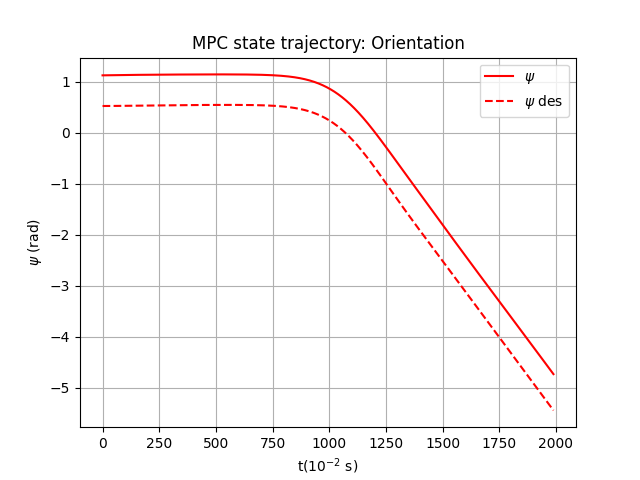
\includegraphics[height=70mm]{figs/_mpc_psi_20.png}	
	\caption{Tracked $\psi$ trajectory with 5-10-20\% relative error on $x_0$}
\end{figure} 

\begin{figure}[!h]
    \center
	\includegraphics[height=70mm]{figs/_mpc_V_5.png}	
	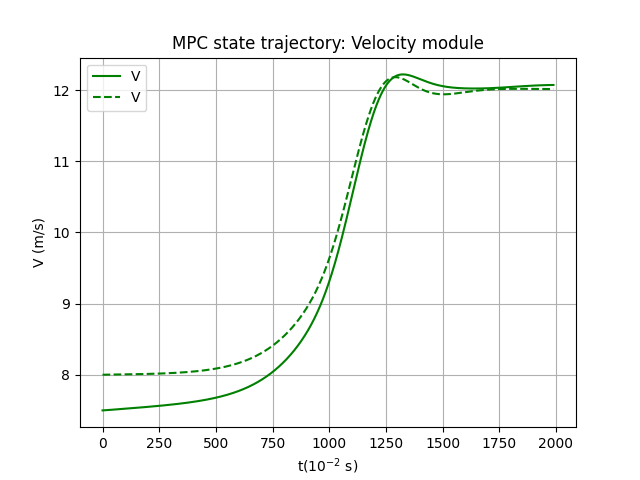
\includegraphics[height=70mm]{figs/_mpc_V_10.png}	
    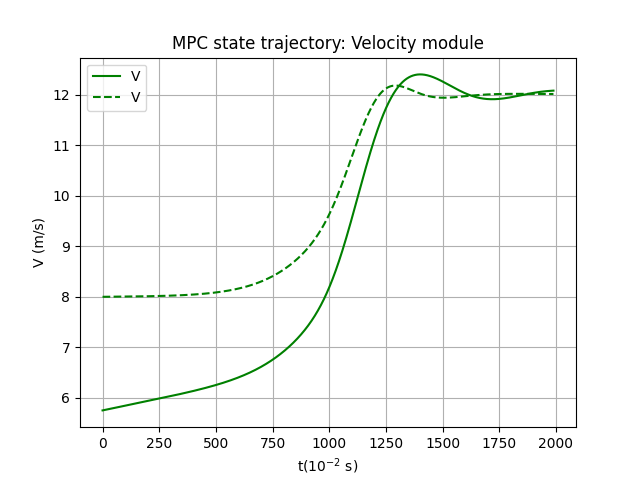
\includegraphics[height=70mm]{figs/_mpc_V_20.png}	
	\caption{Tracked $V$ trajectory with 5-10-20\% relative error on $x_0$}
\end{figure} 

\begin{figure}[!h]
    \center
	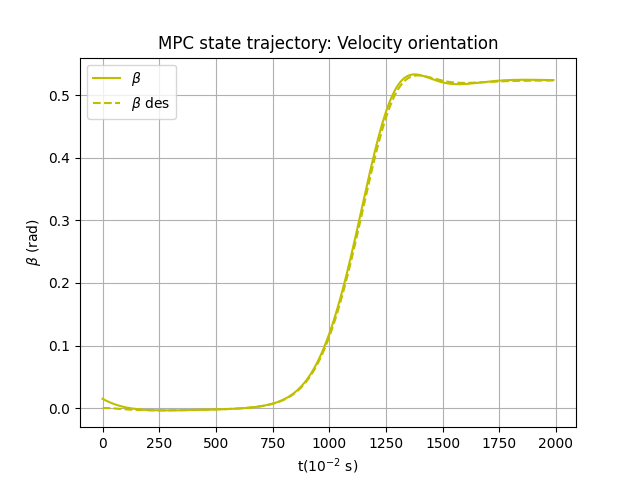
\includegraphics[height=70mm]{figs/_mpc_beta_5.png}	
	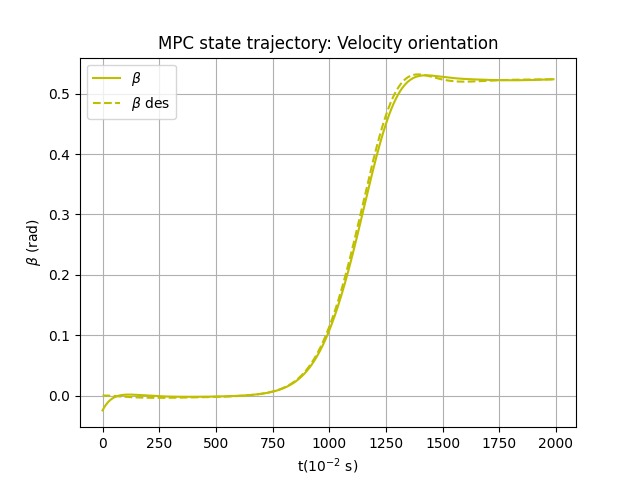
\includegraphics[height=70mm]{figs/_mpc_beta_10.png}	
    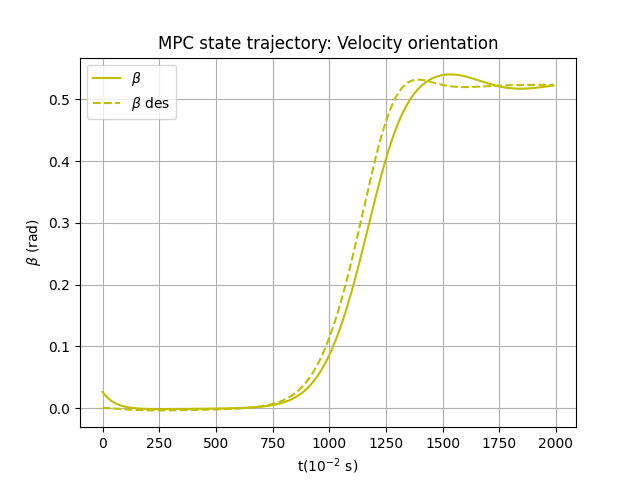
\includegraphics[height=70mm]{figs/_mpc_beta_20.png}	
	\caption{Tracked $\beta$ trajectory with 5-10-20\% relative error on $x_0$}
\end{figure} 

\begin{figure}[!h]
    \center
	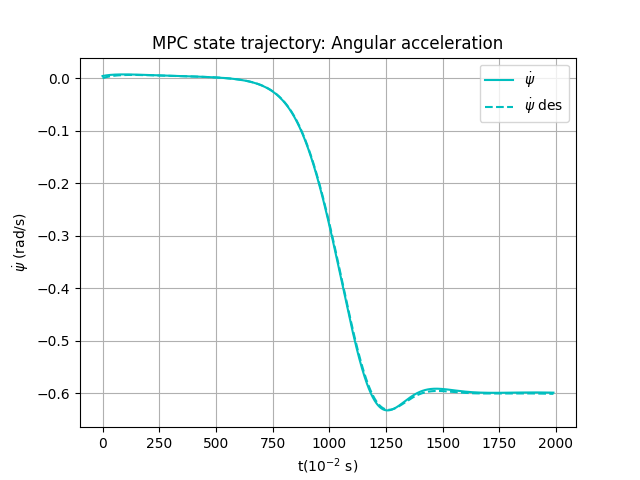
\includegraphics[height=70mm]{figs/_mpc_psidot_5.png}	
	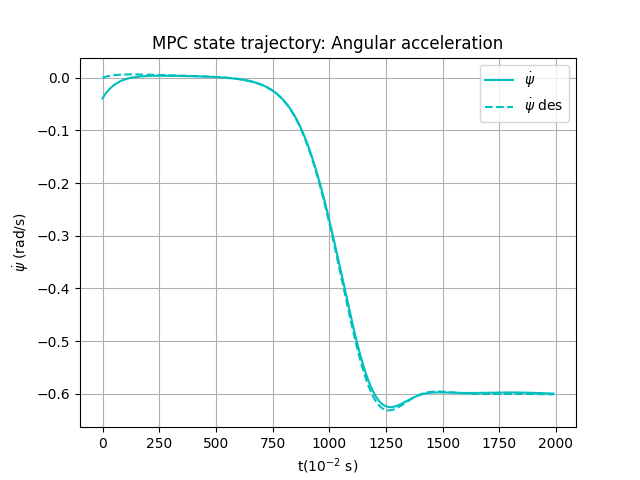
\includegraphics[height=70mm]{figs/_mpc_psidot_10.png}	
    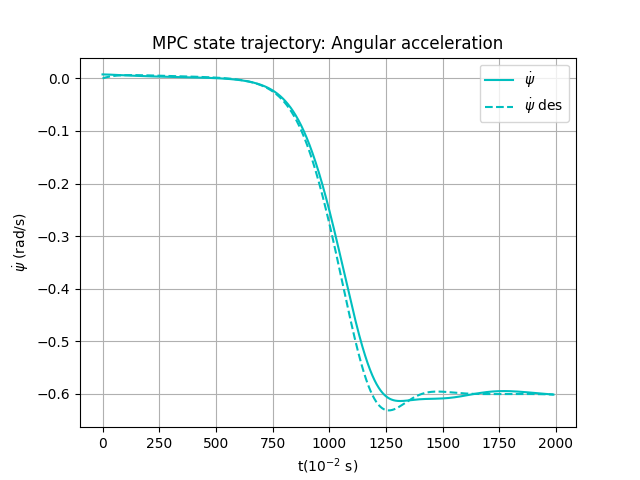
\includegraphics[height=70mm]{figs/_mpc_psidot_20.png}	
	\caption{Tracked $\dot{\psi}$ trajectory with 5-10-20\% relative error on $x_0$}
\end{figure} 

\begin{figure}[!h]
    \center
	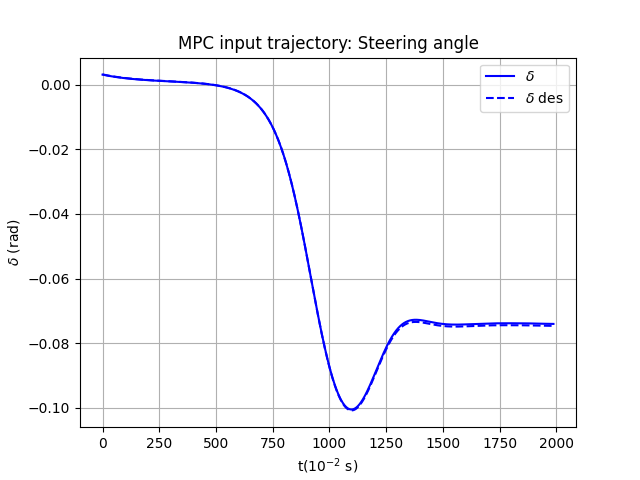
\includegraphics[height=70mm]{figs/_mpc_delta_5.png}	
	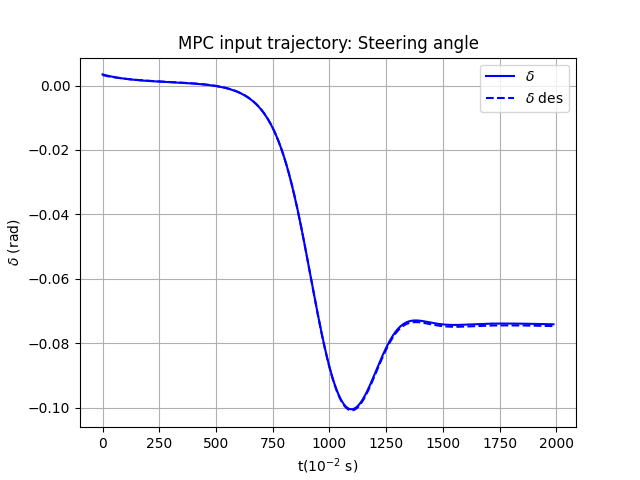
\includegraphics[height=70mm]{figs/_mpc_delta_10.png}	
    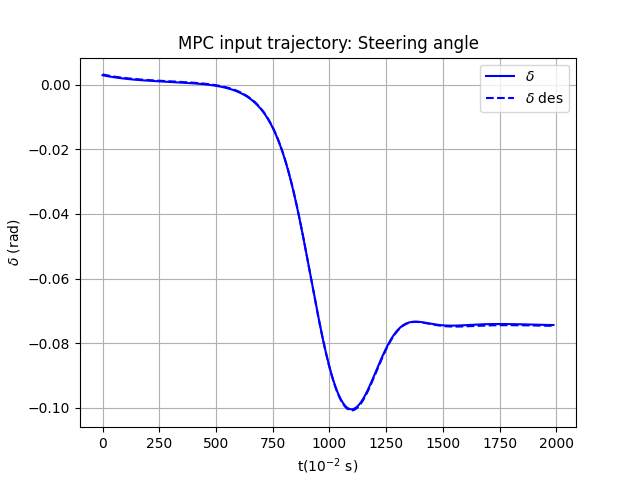
\includegraphics[height=70mm]{figs/_mpc_delta_20.png}	
	\caption{Tracked $\delta$ trajectory with 5-10-20\% relative error on $x_0$}
\end{figure} 

\begin{figure}[!h]
    \center
	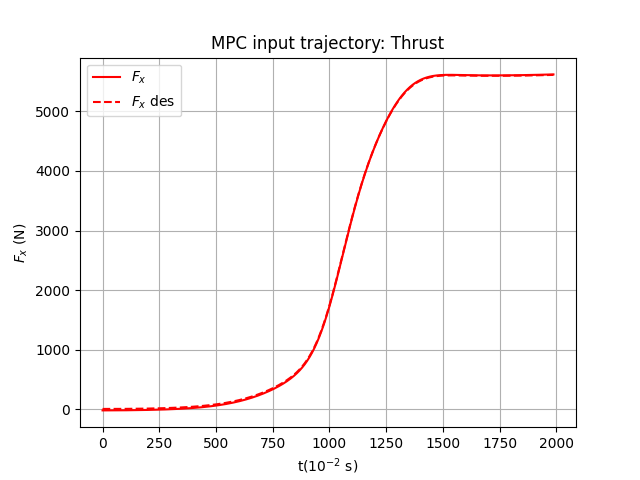
\includegraphics[height=70mm]{figs/_mpc_Fx_5.png}	
	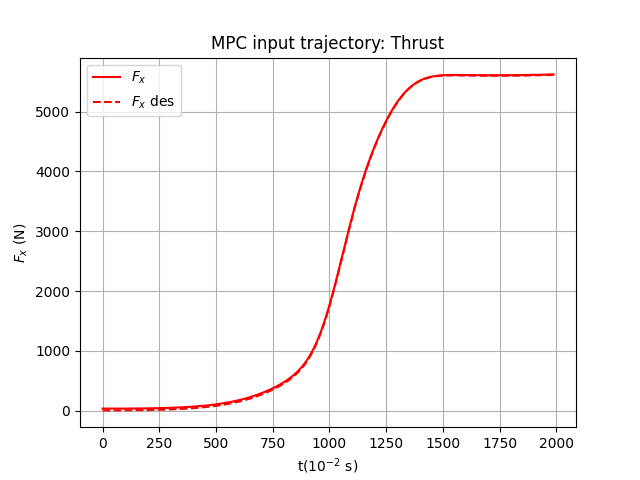
\includegraphics[height=70mm]{figs/_mpc_Fx_10.png}	
    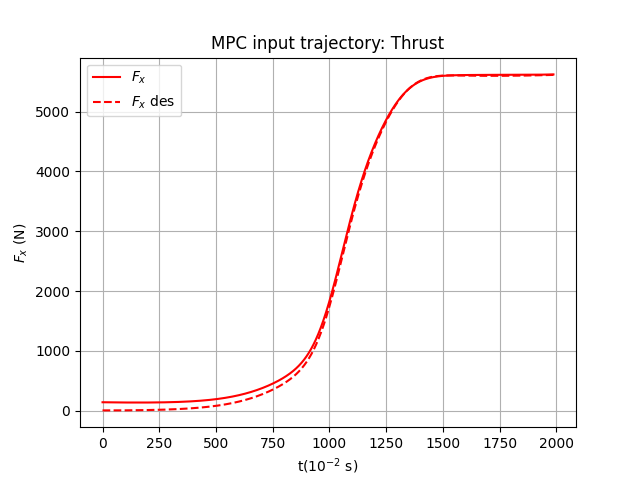
\includegraphics[height=70mm]{figs/_mpc_Fx_20.png}	
	\caption{Tracked $F_x$ trajectory with 5-10-20\% relative error on $x_0$}
\end{figure}

\section{Conclusions}
Altough the performances in tracking the velocities are good, even for a small error on the initial condition we reach considerable errors in the steady state values for the position and orientation variables. This is sensitively reduced when the error is on a single initial state component. We tried to address the problem by increasing the costs on the position variables and reducing the costs on the input but that had little to no result. We also tried with different time horizons $T_{mpc}$ and found 10 time instants to be the best trade off between efficiency for control and computational time. 
Overall, the MPC performances seem to be slightly worse than the LQR ones, but that is explainable via the fact that the LQR gains are computed by taking into account the whole trajectory for the system, while the MPC input takes into account only a small time window.
\chapter{Task 5 - Animation}
In this last task we need to animate the tracking of the optimal trajectory with some initial error as obtained in Task 3.
\\Our best car, Saetta McQueen, is ready to run for us and he is already spitting purple flames to represent the force
$F_x$ (purple because \texttt{forza Viola}).


\begin{figure}[h]
    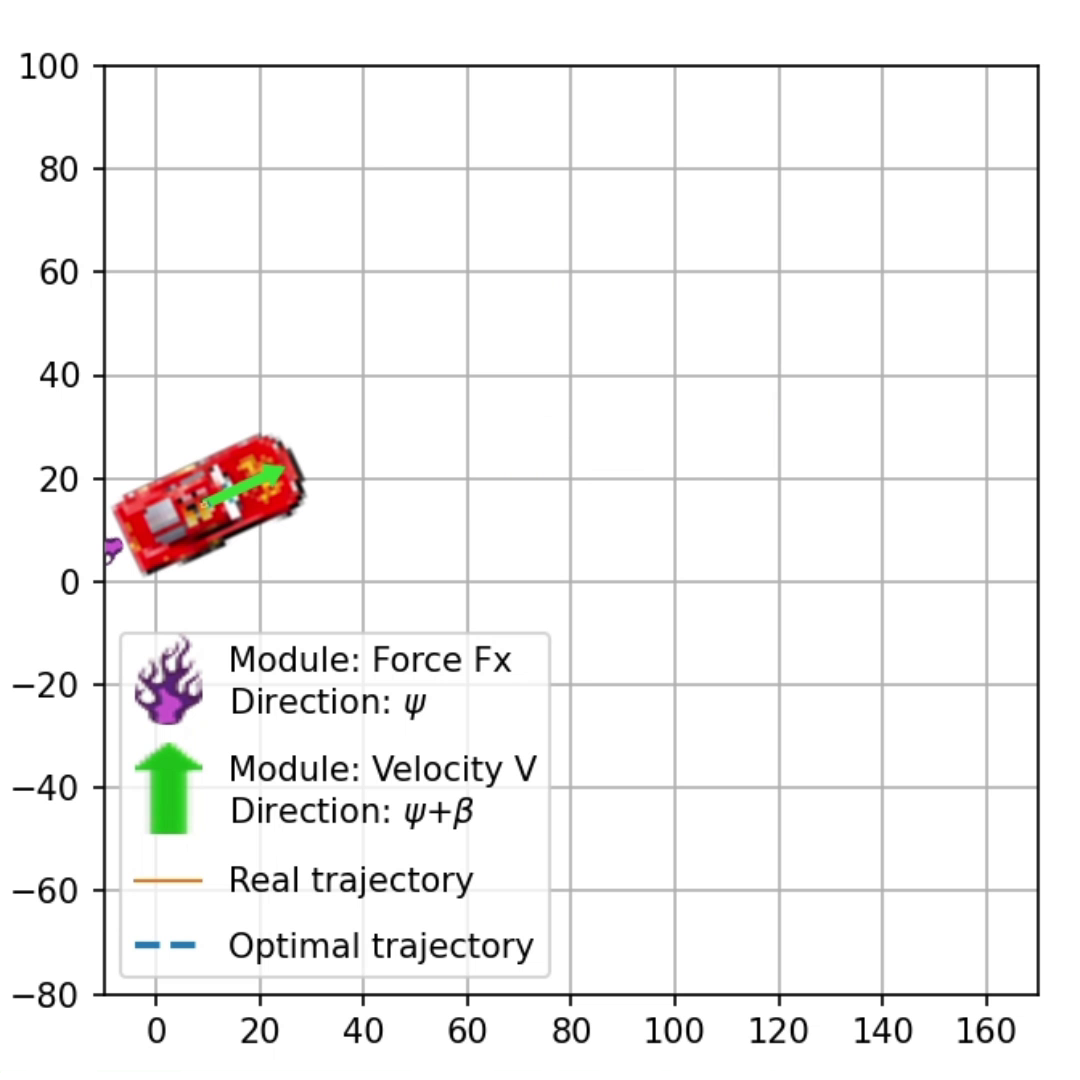
\includegraphics[width=0.5\linewidth]{figs/saetta_video/00001.png}
    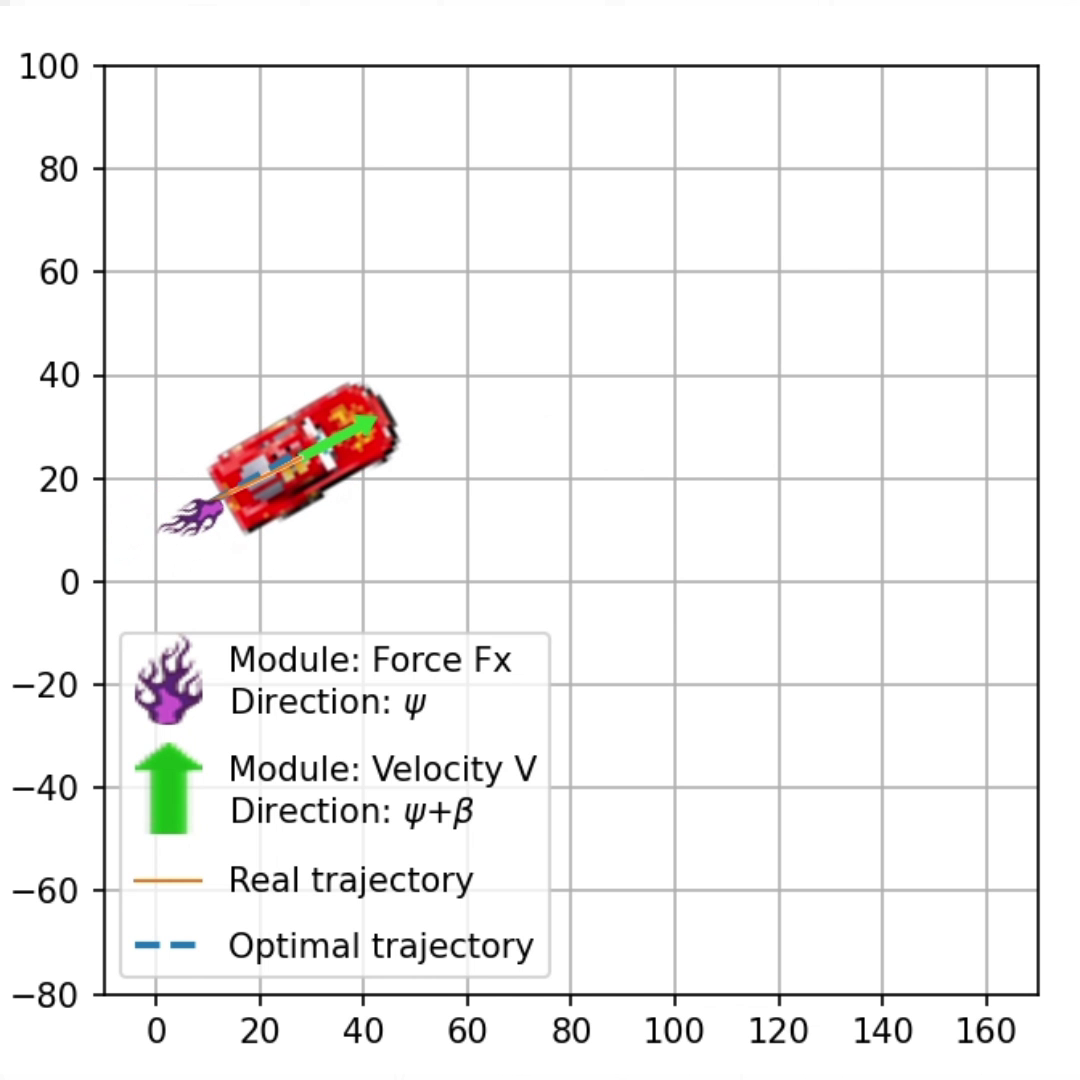
\includegraphics[width=0.5\linewidth]{figs/saetta_video/00080.png}
\end{figure}

\begin{figure}[h]
    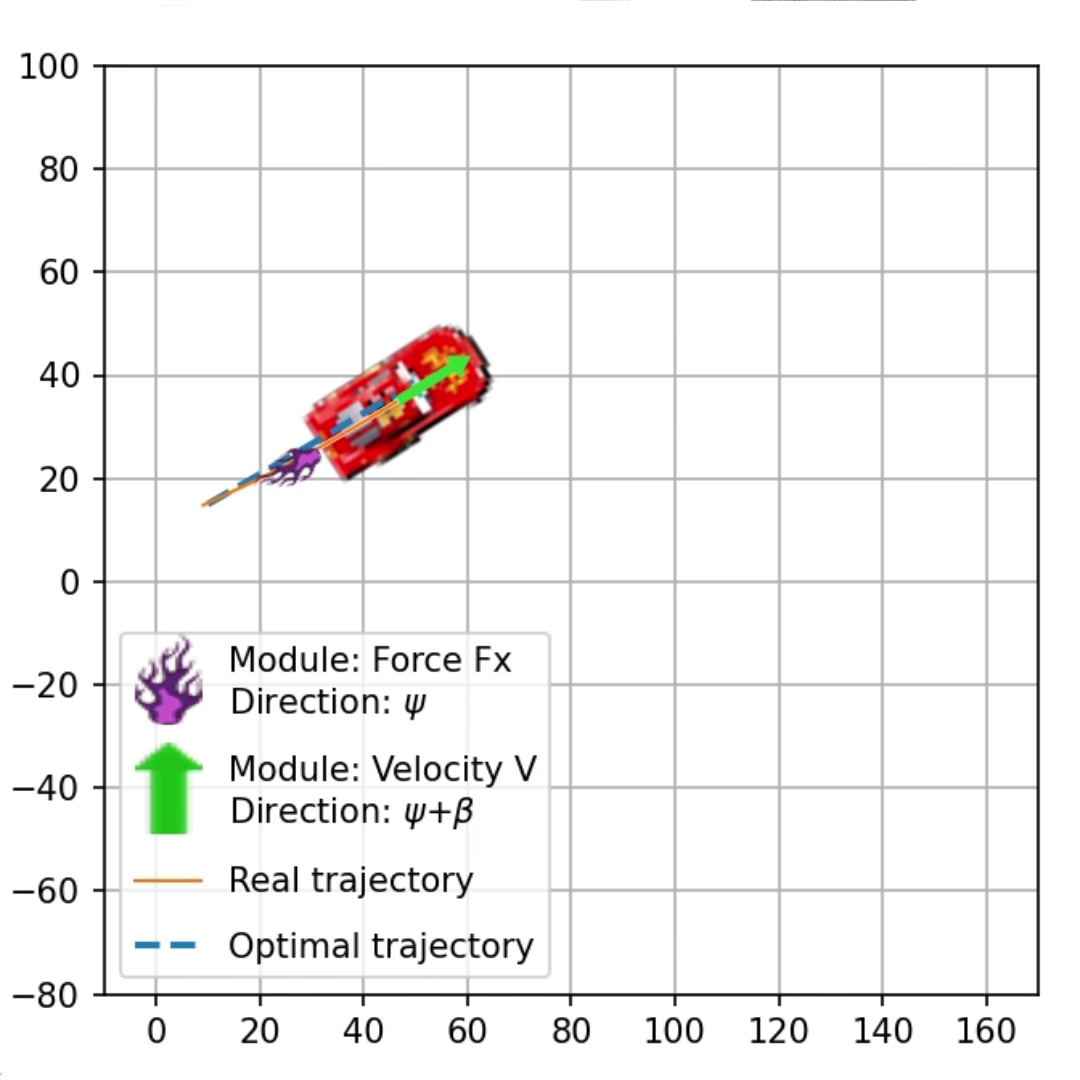
\includegraphics[width=0.5\linewidth]{figs/saetta_video/00160.png}
    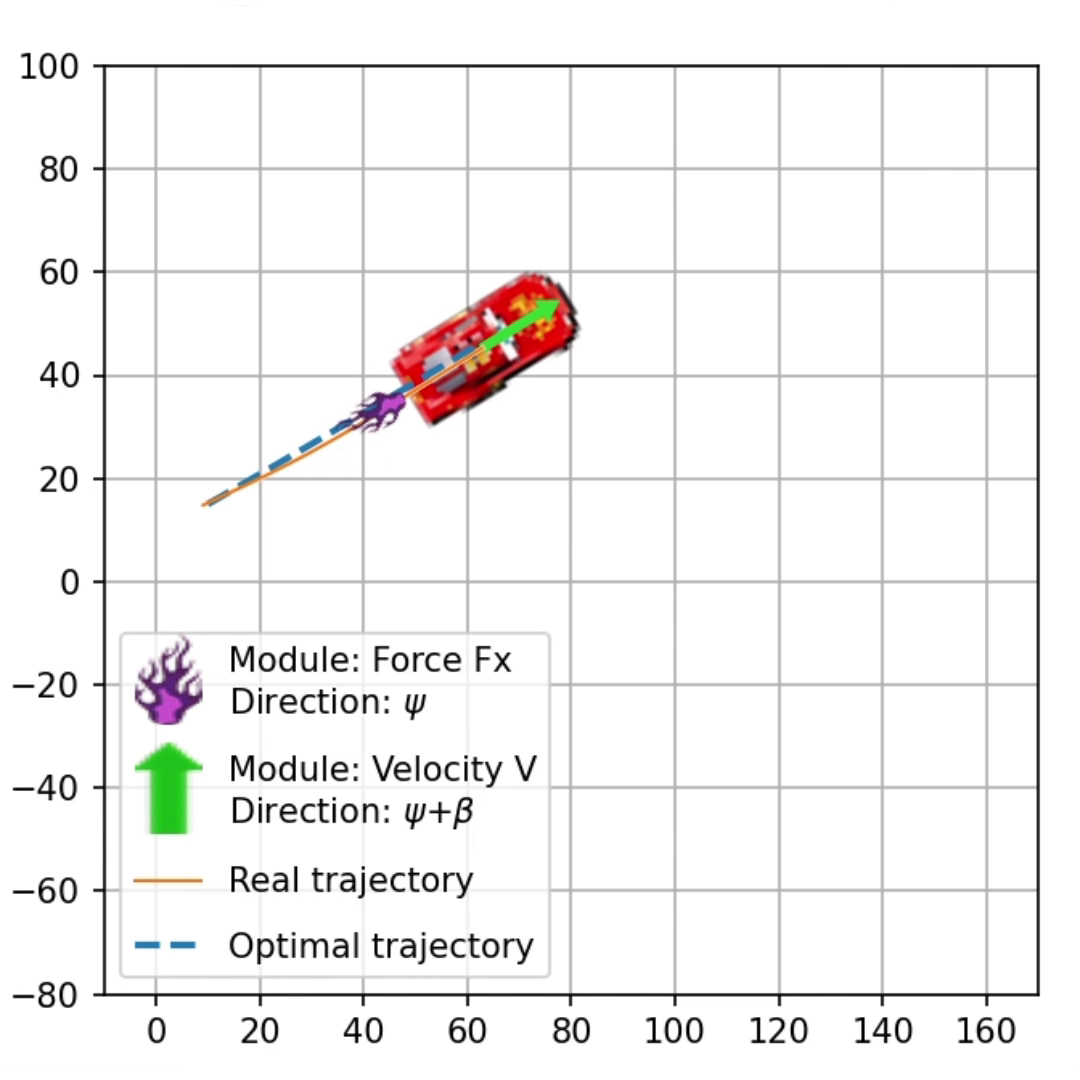
\includegraphics[width=0.5\linewidth]{figs/saetta_video/00240.png}
\end{figure}

\begin{figure}[h]
    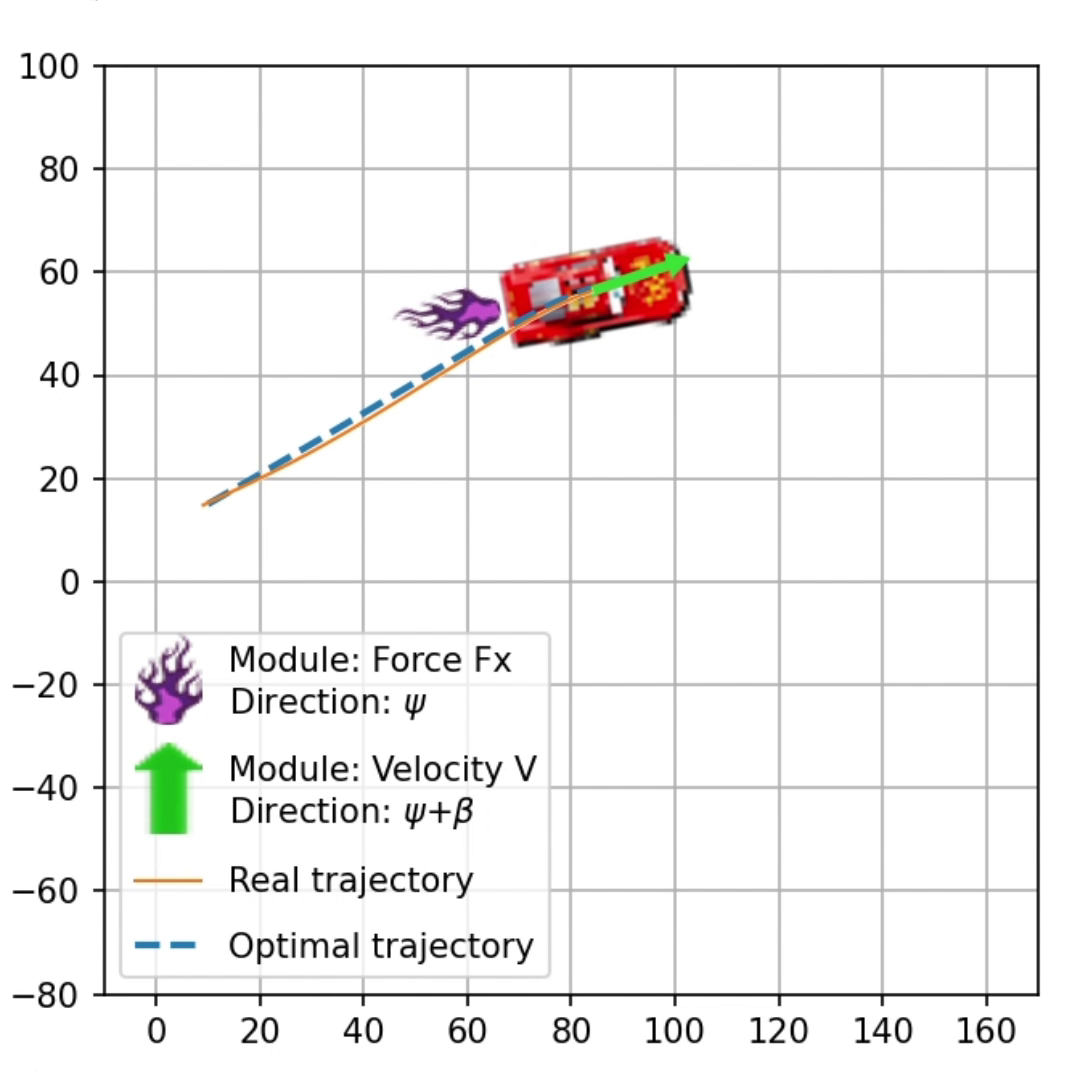
\includegraphics[width=0.5\linewidth]{figs/saetta_video/00320.png}
    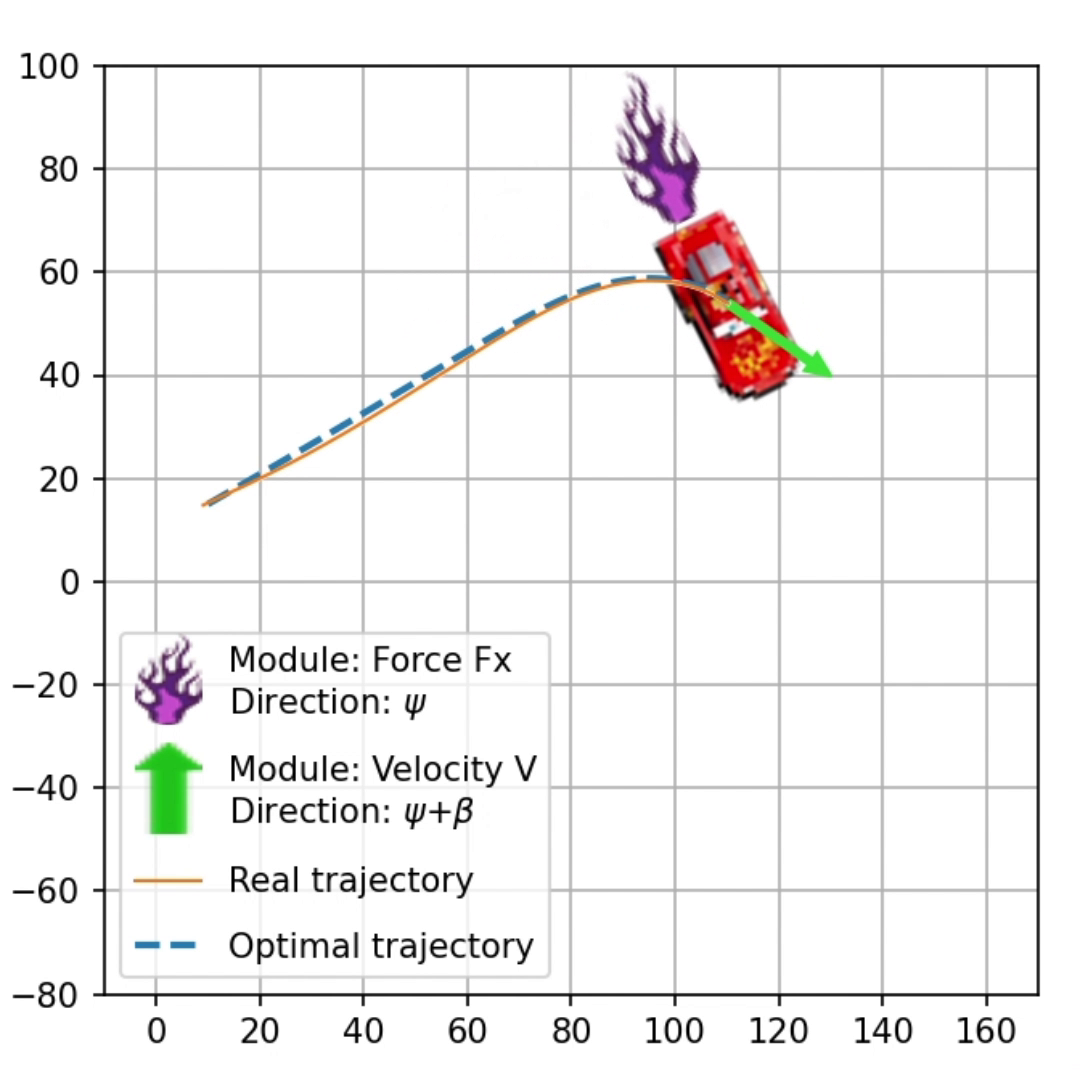
\includegraphics[width=0.5\linewidth]{figs/saetta_video/00400.png}
\end{figure}

\begin{figure}[h]
    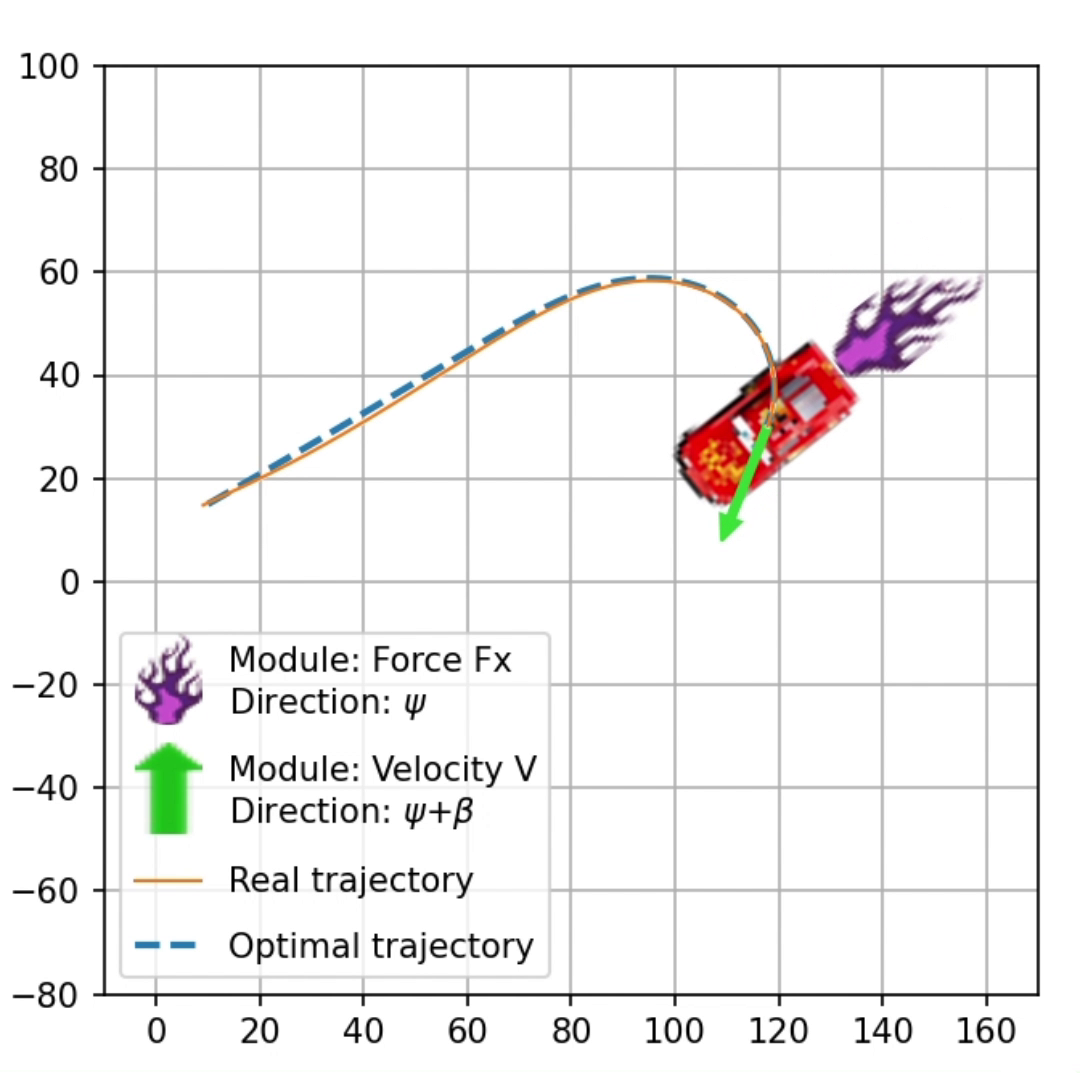
\includegraphics[width=0.5\linewidth]{figs/saetta_video/00480.png}
    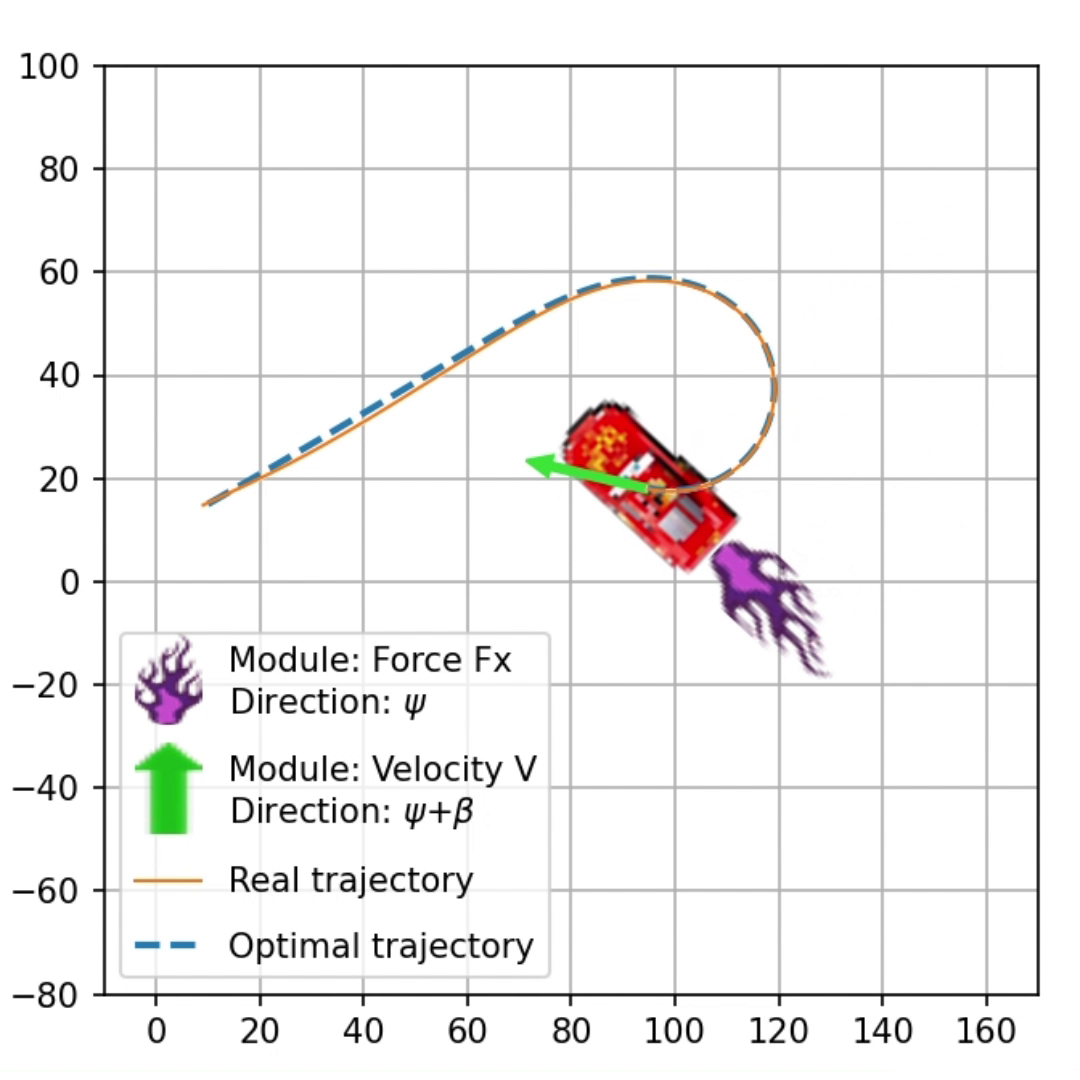
\includegraphics[width=0.5\linewidth]{figs/saetta_video/00560.png}
\end{figure}

\begin{figure}[h]
    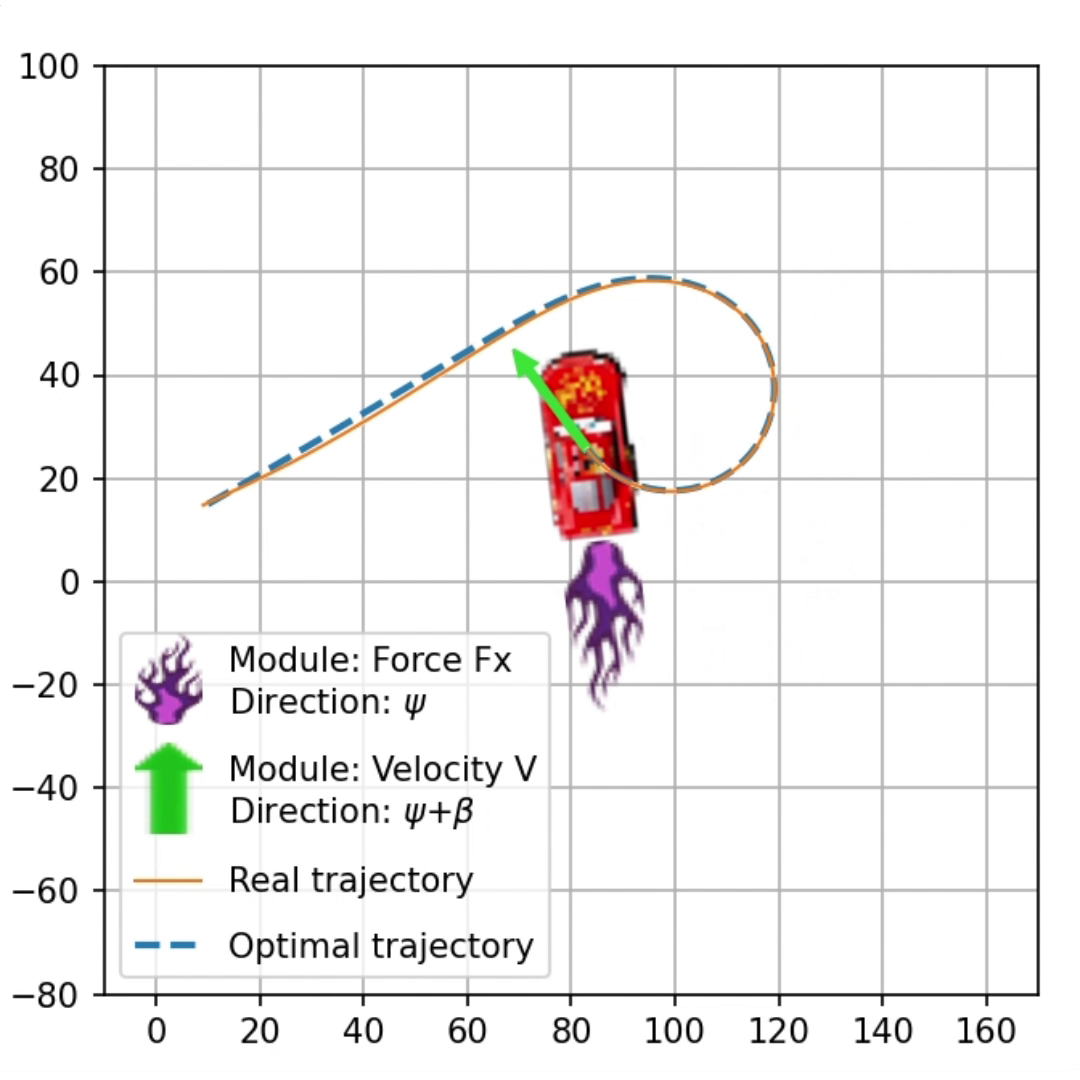
\includegraphics[width=0.5\linewidth]{figs/saetta_video/00600.png}
    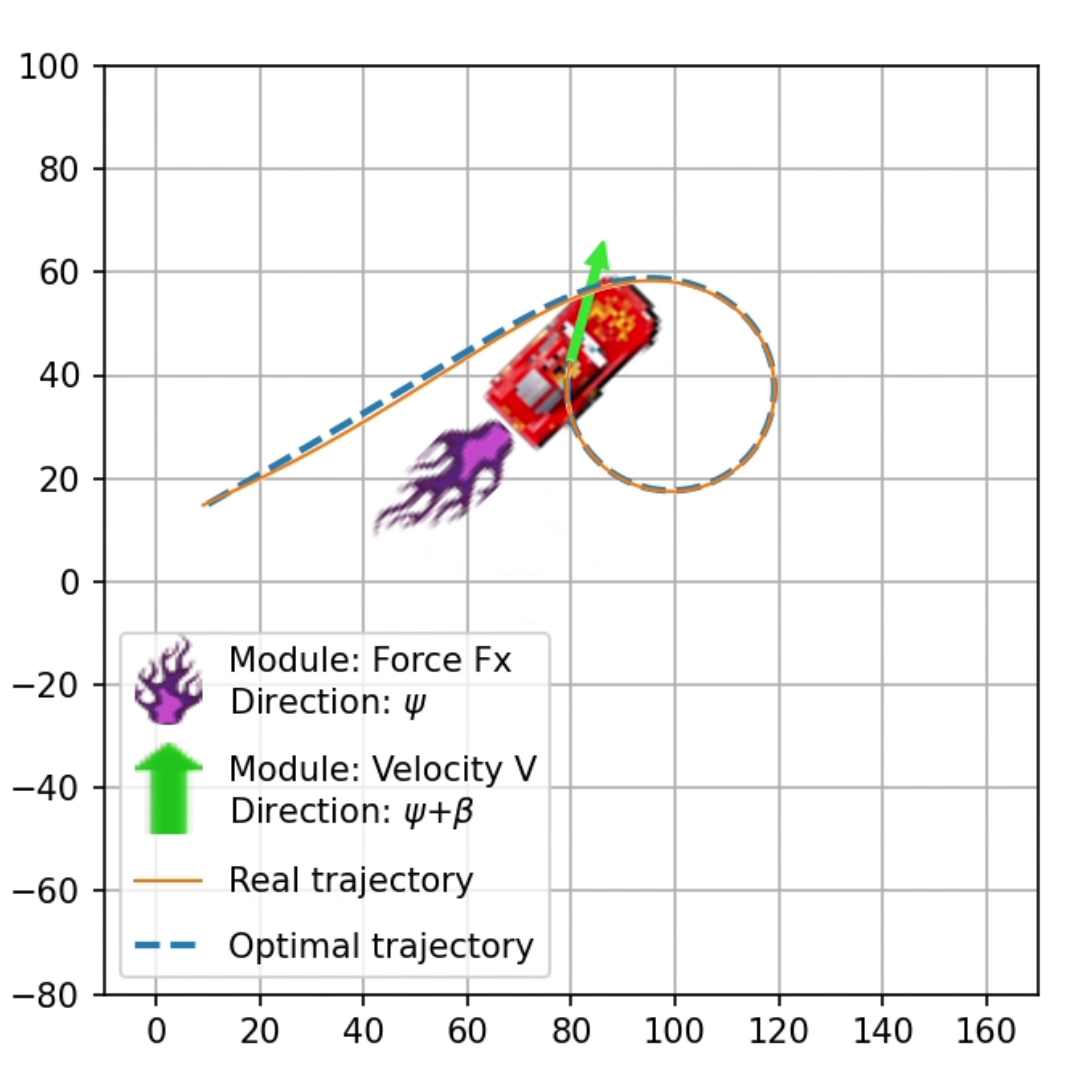
\includegraphics[width=0.5\linewidth]{figs/saetta_video/00649.png}
\end{figure}
%%%%%%%%%% Conclusions %%%%%%%%%%
\chapter*{Conclusions}
\addcontentsline{toc}{chapter}{Conclusions} 
In conclusion this project focused on the use of Python to solve typical optimal control problems.

\bigskip
We modeled the dynamics and the first order derivatives in Task 0 to set-up the problem.\\
In task 1 we computed two cornering equilibria and created a step desired curve with long tails.
We proceeded to use a Newton's approximated algorithm with Armijo's step size selection to compute the optimal 
trajectory.\\
In task 2 we moved to a smooth desired curve and found the results to be better in terms of cost and inputs usage.\\
Tasks 3 and 4 were about controlling with uncertainties around the optimal trajectory and we tested a linear 
quadratic regulator and a model predictive controller to track the obtained smooth trajectory.\\
In task 5 we animated the result obtained in task 3. 
%%%%%%%%%% Bibliography %%%%%%%%%%%
% \bibliography{bibfile}{}
% \bibliographystyle{plain}
% \addcontentsline{toc}{chapter}{Bibliography}

% \nocite{*}
%%%%%%%%%%%%%%%%%%%%%%%%%%%%%%%%%%%%%%


\end{document}